\documentclass[type=bachelor]{thuthesis}
% 选项:
%   type=[bachelor|master|doctor|postdoctor], % 必选
%   secret,                                   % 可选
%   pifootnote,                               % 可选(建议打开)
%   openany|openright,                        % 可选,基本不用
%   arial,                                    % 可选,基本不用
%   arialtoc,                                 % 可选,基本不用
%   arialtitle                                % 可选,基本不用

% 所有其它可能用到的包都统一放到这里了,可以根据自己的实际添加或者删除。
\usepackage{thuthesis}

% 定义所有的图片文件在 figures 子目录下
\graphicspath{{figures/}}

% 可以在这里修改配置文件中的定义。导言区可以使用中文。
\def\myname{周立旺}

\begin{document}

%%% 封面部分
\frontmatter
\thusetup{
  %******************************
  % 注意:
  %   1. 配置里面不要出现空行
  %   2. 不需要的配置信息可以删除
  %******************************
  %
  %=====
  % 秘级
  %=====
  secretlevel={秘密},
  secretyear={10},
  %
  %=========
  % 中文信息
  %=========
  ctitle={黑白视频自动着色算法},
  cdegree={工学硕士},
  cdepartment={软件学院},
  cmajor={软件工程},
  cauthor={周立旺},
  csupervisor={王斌教授},
  %cassosupervisor={陈文光教授}, % 副指导老师
  %ccosupervisor={某某某教授}, % 联合指导老师
  % 日期自动使用当前时间,若需指定按如下方式修改:
  % cdate={超新星纪元},
  %
  % 博士后专有部分
  %cfirstdiscipline={计算机科学与技术},
  %cseconddiscipline={系统结构},
  %postdoctordate={2009年7月——2011年7月},
  %id={编号}, % 可以留空: id={},
  %udc={UDC}, % 可以留空
  %catalognumber={分类号}, % 可以留空
  %
  %=========
  % 英文信息
  %=========
  %etitle={An Introduction to \LaTeX{} Thesis Template of Tsinghua University v\version},
  % 这块比较复杂,需要分情况讨论:
  % 1. 学术型硕士
  %    edegree:必须为Master of Arts或Master of Science(注意大小写)
  %             “哲学、文学、历史学、法学、教育学、艺术学门类,公共管理学科
  %              填写Master of Arts,其它填写Master of Science”
  %    emajor:“获得一级学科授权的学科填写一级学科名称,其它填写二级学科名称”
  % 2. 专业型硕士
  %    edegree:“填写专业学位英文名称全称”
  %    emajor:“工程硕士填写工程领域,其它专业学位不填写此项”
  % 3. 学术型博士
  %    edegree:Doctor of Philosophy(注意大小写)
  %    emajor:“获得一级学科授权的学科填写一级学科名称,其它填写二级学科名称”
  % 4. 专业型博士
  %    edegree:“填写专业学位英文名称全称”
  %    emajor:不填写此项
  %edegree={Doctor of Engineering},
  %emajor={Computer Science and Technology},
  %eauthor={Xue Ruini},
  %esupervisor={Professor Zheng Weimin},
  %eassosupervisor={Chen Wenguang},
  % 日期自动生成,若需指定按如下方式修改:
  % edate={December, 2005}
  %
  % 关键词用“英文逗号”分割
  ckeywords={黑白视频, 自动着色, 深度网络,CNN, GAN},
  ekeywords={Black and white video, Automatic colorization, Deep network, CNN, GAN}
}

% 定义中英文摘要和关键字
\begin{cabstract}
  黑白图像着色是个由来已久且研究得较为成熟的课题,这个课题的任务是将输入的黑白图
  像还原出它的色彩信息,是图形学领域的一个经典问题。在深度学习普及之前,普遍使用
  的方法是通过人为指定一些局部颜色信息,然后用最优化的方法补全颜色。而最近几年随
  着深度学习的广泛应用,许多研究也用深度学习的方法在黑白图像着色问题上做到了自动
  化,而不需要人工干涉,得到的结果也非常不错。

  黑白视频着色问题相比图像着色问题更难,相关的研究也更少。传统的通过人工干涉的最
  优化方法有对视频着色的研究,通过将最优化目标由二维扩展到三维上做到;但现在还没
  有考虑时间连续性的全自动的黑白视频着色算法,这就是本文的研究目标。

  在这篇论文中,我训练了多种对黑白图像着色的GAN模型,训练了多种对视频关键帧着色
  的GAN模型,处理了视频关键帧之间黑白帧的着色问题。
\end{cabstract}

% 如果习惯关键字跟在摘要文字后面,可以用直接命令来设置,如下:
% \ckeywords{\TeX, \LaTeX, CJK, 模板, 论文}

\begin{eabstract}
   As one of the basic tasks in computer graphics, Black and white image colorization has been a long exist and fully researched task, which aims to restore color information of a gray input image. Before deep learning has been widely applied, a tranditional solution to this problem is using optimization, with local color information manually offered, called user-guided colorization. while with the development of deep learning these years, many new methods have been raised, which deals with automatic image colorization and reaches the state-of-art.

   Comparing to image colorization, Black and white video colorization is a harder and less researched problem. Tranditional way of optimization with manual hints can do this by appling 2D objective function to 3D. While there are no mature fully automatic methods of video colorization concerning about time consistency, this paper tries to find a solution.

   In this paper, I train many image colorization and video key-frames colorzation models based on GAN. Except for that, I also deal with task of colorizing inter-frames between key-frames.

\end{eabstract}

% \ekeywords{\TeX, \LaTeX, CJK, template, thesis}

% 如果使用授权说明扫描页,将可选参数中指定为扫描得到的 PDF 文件名,例如:
% \makecover[scan-auth.pdf]
\makecover

%% 目录
\tableofcontents

%% 符号对照表
\begin{denotation}[3cm]
\item[CNN] 卷积神经网络 (Convolutional Neural Network)
\item[GAN] 生成对抗网络 (Generative Adversarial Network)
\item[ANN] 人工神经网络 (Artificial Neural Network)
\end{denotation}



%%% 正文部分
\mainmatter
\chapter{引言}
\label{cha:intro}

\section{课题背景、目的和意义}
\label{sec:intro}

  黑白图像着色是个由来已久且研究得较为成熟的课题,这个课题的任务是将输入的黑白图
  像还原出它的色彩信息,是图形学领域的一个经典问题。在深度学习普及之前,普遍使用
  的方法是通过人为指定一些局部颜色信息,然后用最优化的方法补全颜色。而最近几年随
  着深度学习的广泛应用,许多研究也用深度学习的方法在黑白图像着色问题上做到了自动
  化,而不需要人工干涉,得到的结果也非常不错。

  传统的非深度学习方法例如~\inlinecite{journals/tog/LevinLW04},通过人工输入一些区域的彩色条带,根据全图的灰度信息来最优化填充剩余位置的颜色信息。而深度学习的方法例如~\inlinecite{IizukaSIGGRAPH2016}、~\inlinecite{zhang2016colorful}均是通过训练神经网络的方式来进行自动上色。~\inlinecite{IizukaSIGGRAPH2016}训练了一个多层次的CNN,结合提取的局部特征与全局信息来对整张图着色。~\inlinecite{zhang2016colorful}使用的是单层次的CNN,但选择了特别的损失函数:考虑到使用欧式距离作为损失函数会使得神经网络将训练集中见过的一类物体所有可能颜色的平均值作为这类物体着色的输出,从而得到失真、灰褐色的结果。所以他们的网络对图片的每个像素输出一个所有颜色离散化后的概率分布,然后从整张图的颜色概率分布中得出一个空间连续的结果。

  然而,虽然黑白图像着色的问题已经研究得比较成熟了,但关于这个问题在时间维度的扩展问题——即黑白视频着色的研究却甚少,现在还没有全自动的黑白视频着色方法。~\inlinecite{journals/tog/LevinLW04}中除了用人工输入结合最优化的方法对黑白图像着色进行了处理,还将最优化的目标通过光流扩展到了时间维度,处理了黑白视频着色,取得了不错的结果。但是在深度学习火热的今天,还没有人提出全自动的方法来处理黑白视频着色问题。

  本文对黑白视频着色问题进行了研究,尝试通过深度学习的提出一个不需要人工干预的全自动的方法来解决这个问题。

\section{主要工作与创新}
\label{sec:works}

  本文的主要工作是为黑白视频着色问题提供一个全自动的解决方案,填补当前这个问题上的空白。

\subsection{图像着色}
\label{sec:image-color}

  在直接进行视频着色前,为了验证所选模型的可行性,先构建了一个处理2D图像的网络模型在图像数据集上训练验证。

  本文选择的深度网络模型是GAN(对抗生成网络)。该模型的思想为同时训练两个模型,生成器和判别器,训练过程中我们将黑白图像输入给生成器,期望它输出理想的着色结果即彩色图像,而我们会将生成器生成的假的彩色图像与真实的彩色图像混在一起交给判别器,期望判别器能分辨出哪些是真的彩色图像,哪些是生成器生成的图像,这样两个网络之间就存在一种对抗关系:生成器要不断学习骗过判别器,而判别器也要学习将真假图像分辨出来。这样当两个网络不断迭代,到判别器也很难分辨出假的生成图像后,训练好的生成器就能拿来做图像生成了。

\subsection{视频着色}
\label{sec:video-color}

  在图像着色的问题上验证好了网络的可行性后,便可将对抗生成网络从处理2D图像扩展到3D视频。具体做法是将生成器与判别器两个网络的卷积核,都在原来处理二维图像的基础上添加新的一维,即是做三维的卷积,使得网络每一层都是对多帧多通道图像做处理,从而达到视频处理的目的。

  在这里,我们尝试过将整个视频每一个连续帧都放进网络做训练,后来发现这样会有几个问题:每个视频的帧数是不一样的,而网络在做卷积的三个维度(宽,高,帧数)上都是固定的,这样只能将视频分为几个帧数固定的段,分别通过网络着色后再合并,而这样又引出了段间合并的连续性问题;另外将网络从2D扩展到3D后,网络参数出现了很大的增长,如果使用连续帧的话,这个问题更加明显,后果就是网络训练变得非常慢,而训练效果也很不理想。

  基于以上的原因,我们采取了关键帧着色的方式,即对于待着色视频,按某种方式取出一定帧数的关键帧,用网络将这部分关键帧着色后,再以最优化的方式给关键帧之间的图像着色。

\subsection{帧间处理}
\label{sec:interframes}

  在得到关键帧的着色后,就要对关键帧之间未着色的图像进行着色,着色的依据便是已有的关键帧颜色。

  对于两个关键帧之间的黑白帧,我们采取递推的方式着色,用前一帧作为后一帧测参考来给后一帧着色,后一帧着色后又可以作为它的后一帧的参考,以此类推。在两个相邻帧之间的着色过程如下:计算两帧之间的光流,对于后一帧的每个像素,在前一帧的光流对应点附近以及与它同坐标位置的点附近,找一个灰度最接近的点,取这个点的颜色作为待着色点的颜色。这样处理后必定会有许多不正常的颜色点,所以后续还需要一些颜色修正以及帧间灰度连贯性的处理。

\subsection{数据集的选择}
\label{sec:dataset}

  在图像着色上,我们使用了小容量的LSUN、CIFAR10以及大容量的Image-Net数据集;在视频着色上,我们使用了UCF11和UCF101等用于动作识别的数据集。

\section{论文的组织与安排}
\label{sec:org}

  本文的其他章节安排如下:

  第二章介绍了本文的相关工作和预备知识,包括卷积神经网络与对抗生成网络的概念。

  第三章介绍了我们的网络结构以及相关算法,包括图像着色与视频着色分别的生成器网络和判别器网络,以及用于帧间处理的最优化算法。

  第四章展示了我们的实验结果,分析了实验结果好的原因,也对坏的结果做了分析。

  第五章总结了我们的工作,并且对未来的工作做了进一步规划。
\chapter{相关工作与预备知识}
\label{cha:2-related}

  与本文研究内容相关的工作主要包括两个方面:黑白图像着色与生成对抗网络。我们将介绍这两个方面的相关工作和本文需要的预备知识。

\section{黑白图像着色}
\label{sec:2-image-color}

  黑白图像着色问题的研究以深度学习的兴起作为分界点分为两个阶段:计算机辅助阶段与计算机全自动阶段,而这两个阶段中的研究重点,研究方法以及效果也是差异很大。

\subsection{计算机辅助的图像着色}
\label{sec:2-user-guided-color}
  
  着色是Wilson Markle在1970年提出的一个术语,用于描述给黑白视频或电视节目添加颜色的计算机辅助的过程。之后这个术语被推广到了所有给单色调图像视频添加颜色的范围。

  最早期的着色完全依赖人工,主要问题在于非常耗时耗力。艺术家要给一张黑白图像着色,先要将它划分为多个区域,然后给每个区域分别指定颜色。分割的过程也可以让计算机自动来做,但分割算法的问题在于无法处理一些复杂的、迷惑的区域边界,比如人的头发和脸。视频的着色还需要追踪区域在帧与帧之间的移动,而现有的追踪算法对于非刚性物体不能稳定追踪。这些问题都会导致人工工作量的增加。

  2003年的一款给静态图片着色的商业软件BlackMagic,给用户提供了有用的画刷和调色板,但分割的任务还是完全由用户完成。

  Welsh~\cite{DBLP:journals/tog/WelshAM02}等人在2002年提出了一种半自动的着色方法,通过将待着色的灰度图像转换成一张给定彩色图像的颜色风格。他们检测灰度图像中每个像素及其领域的灰度值,着色为被参考的彩色图像中灰度对应领域的颜色。效果如图~\ref{fig:transfer}所示。但是这种方法的问题在于对两张图像区域之间的风格相似度要求很高,所以需要一些人工工作量;另外这个方法也没有显式的保证被着色图像颜色的空间连续性。

  \begin{figure}[H]
    \centering
    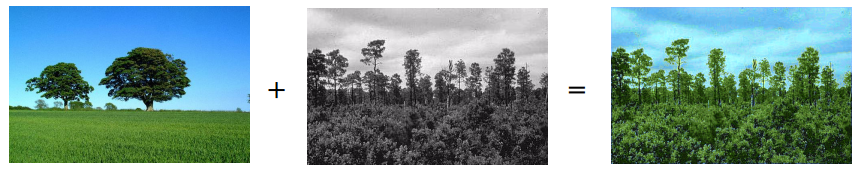
\includegraphics[width=0.7\paperwidth]{transfer_color}
    \caption[Welsh等人的风格转换着色]{Welsh等人的风格转换着色。左边是选择的参考彩色图像,中间是待着色图像,右边是风格转化结果}
    \label{fig:transfer}
  \end{figure}

  Levin~\cite{journals/tog/LevinLW04}等人的方法避开了区域分割的问题,他们做了这样的假设:在时间、空间上连续的并且有着相似灰度的像素应该最终是相似的颜色。在这个假设的基础上,他们设计了一个二次损失函数并将这个问题转换成了一个标准化的最优化问题。他们的输入时认为指定的一些彩色条带,如图~\ref{fig:color_optim}所示,最优化的目标即是在这些已知颜色的像素基础上,最小化相似灰度相邻像素的颜色差。

  \begin{figure}[H]
    \centering
    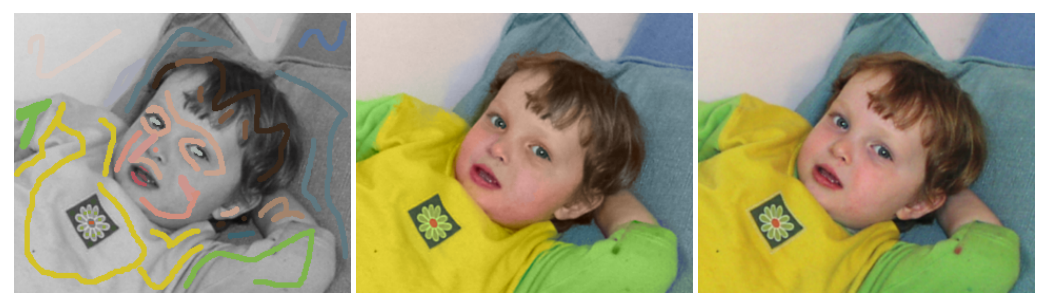
\includegraphics[width=0.7\paperwidth]{color_optim}
    \caption[Levin等人的最优化着色]{Levin等人的最优化着色。左边是人工添加的彩色条带提示,中间是着色结果,右边是原始真实图像}
    \label{fig:color_optim}
  \end{figure}

  不过以上这些计算机辅助着色都有的问题就是需要人工根据经验指定一些区域或像素的颜色,无法完全解放人力。

\subsection{计算机全自动的图像着色}
\label{sec:2-automatic-color}

  随着机器学习与深度学习席卷计算机图像、计算机视觉领域的各个研究方向,也出现了许多关于着色问题的数据驱动方法的研究。

  Cheng~\cite{DBLP:journals/corr/ChengYS16}等人训练了一个神经网络来处理着色。基于学习的着色的基本思路都是:对于数据集中的真实彩色图像,将其变换到LAB或者YUV等个通道、灰度与色度独立的颜色空间,将L空间或者Y空间作为网络输入,而AB或者UV作为真实值,目标就是最小化网络输出与真实值之间的差异。Cheng~\cite{DBLP:journals/corr/ChengYS16}的处理是,对于输入的灰度图像,通过人工设计的特征提取函数得到图像特征,将这个图像特征作为一个包含三个隐含层的神经网络的输入,得到与原图等大的色度图。由于神经网络直接生成的色度图会存在一些不真实点和空间上的颜色不连续性,于是与原始的灰度输入做一个双线性插值得到一个修正后的色度图,然后将灰度图与色度图结合在一起就可以得到着色后的彩色图像。图~\ref{fig:deep_color}就是这篇论文算法的大致流程。

  \begin{figure}[H]
    \centering
    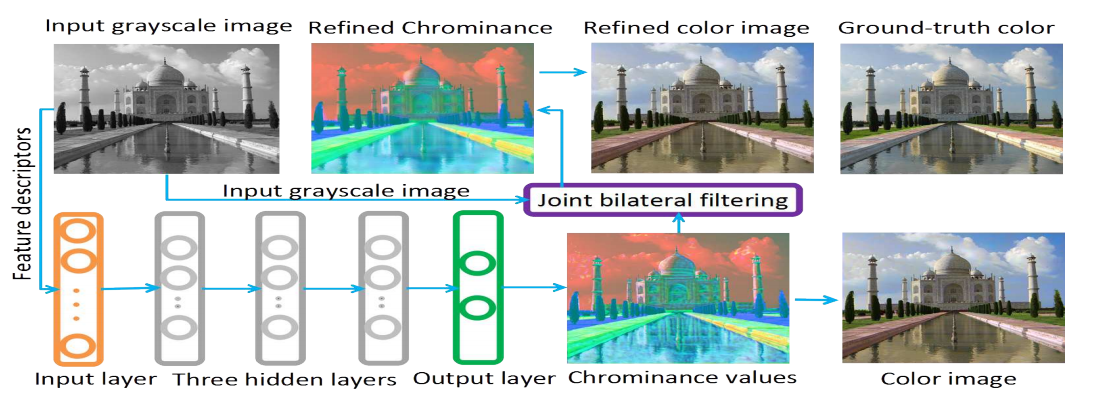
\includegraphics[width=0.7\paperwidth]{deep_color}
    \caption{Cheng等人的算法流程}
    \label{fig:deep_color}
  \end{figure}

  早期神经网络的一个难题就是特征都是人工选取的,特征的效果好坏都需要通过实验说明,而且基于经验的特征选择也是很有限的,只会使用那些经过实验证明可用的特征;另外一点就是能够处理的数据量很有限。Cheng~\cite{DBLP:journals/corr/ChengYS16}的这篇论文也是有很大篇幅在比较各种特征提取函数的效果好坏,图~\ref{fig:feature_choose}给出了他们的一些特征效果的比较。

  \begin{figure}[h]
    \centering
    \subcaptionbox{左图为灰度输入,中间为没有区域特征时的着色,右边是添加了区域特征的结果\label{fig:feature_sub1}}
      {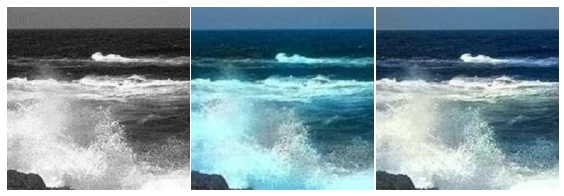
\includegraphics[width=0.3\paperwidth]{feature_sub1}}
    \hspace{4em}
    \subcaptionbox{左图为灰度输入,中间为添加了区域特征和DAISY特征的着色,右边是添加了语义信息特征的着色结果\label{fig:feature_sub2}}
        {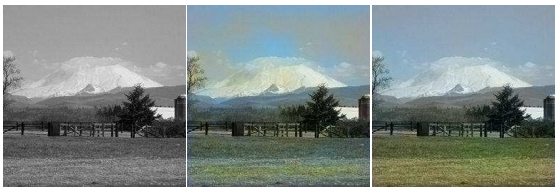
\includegraphics[width=0.3\paperwidth]{feature_sub2}}
    \caption{Cheng论文中的特征选择与比较}
    \label{fig:feature_choose}
  \end{figure}


  CNN的出现就抛弃了人工特征选取的过程,而是一个端到端的训练过程。设计好网络结构以后,以灰度图像直接作为输入,色度图像直接作为输出,经过训练就可以得到直接可用的模型。CNN与ANN在结构上的很大一点不同在于,ANN的相邻两层神经元之间每两个神经元都有信息传递关系,而CNN的相邻两层之间只有空间相邻的神经元才有信息传递,并且同一层的神经元权值共用。这样CNN就可以达到比ANN更深的网络层数和使用更大的数据量,因为它处理的是局部的信息。

  Iizuka~\cite{IizukaSIGGRAPH2016}等人设计了一个更大的CNN网络,并且在更大的数据集ImageNet~\cite{DBLP:journals/ijcv/RussakovskyDSKS15}上进行了训练。他们的核心在于将局部特征与与全局特征进行了结合:局部特征由分辨率较高的卷积层得到,而全局特征由局部特征进一步卷积得到,然后通过一个融合层将局部特征与全局特征结合在一起。得到结合后的特征后,再输入到着色网络,经过一些反卷积层,得到着色结果,最后将着色结果上采样到原图像分辨率结合灰度图就得到彩色图像。图~\ref{fig:let_it_color}即是他们整体的网络结构。

  \begin{figure}[H]
    \centering
    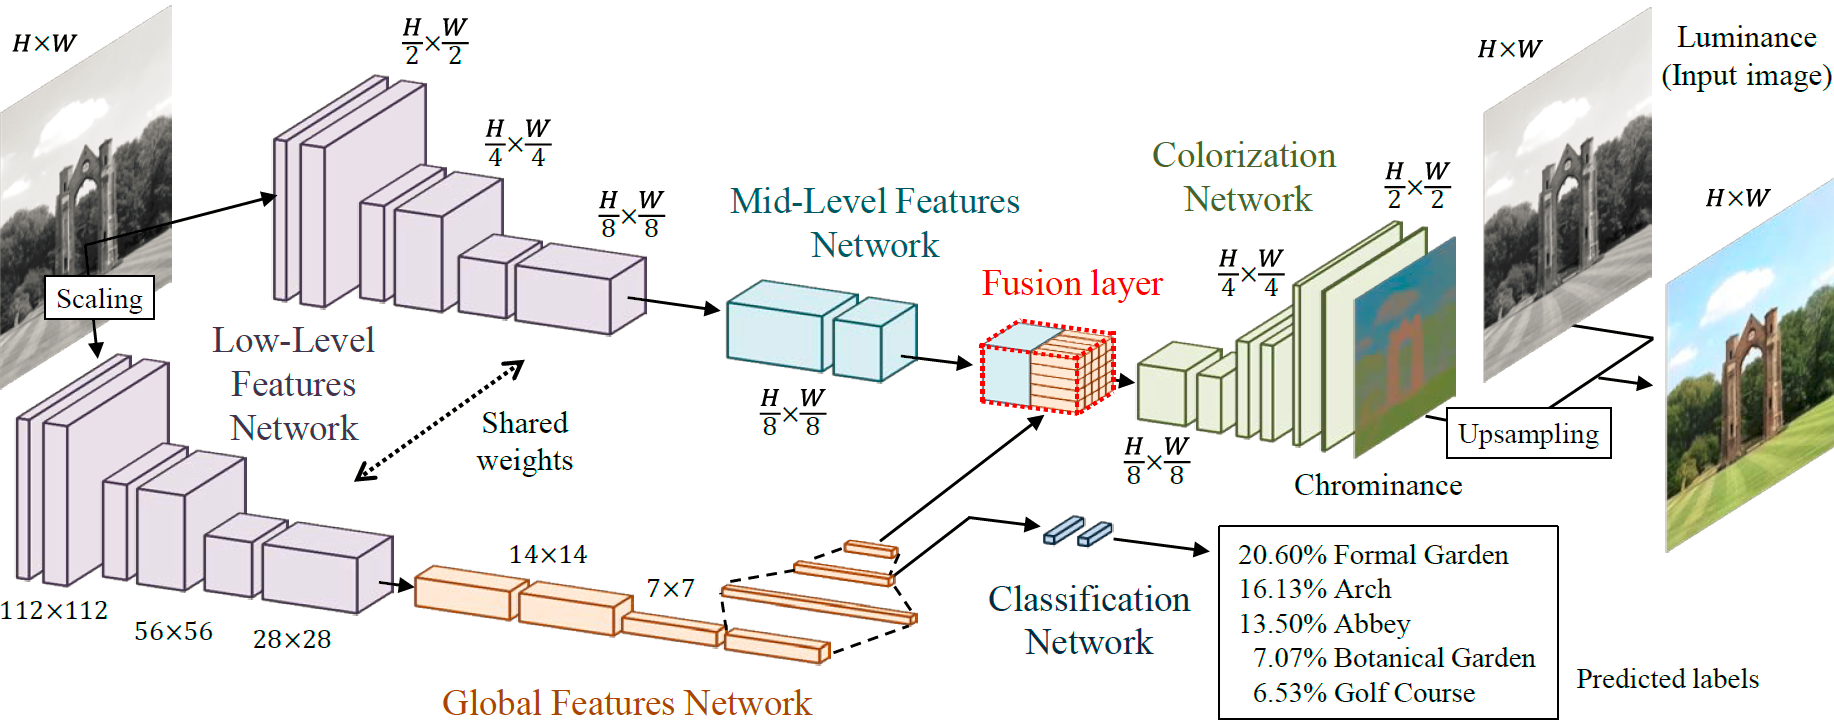
\includegraphics[width=0.7\paperwidth]{let_it_color}
    \caption{Iizuka等人的网络结构}
    \label{fig:let_it_color}
  \end{figure}

  Zhang~\cite{zhang2016colorful}等人从损失函数的角度做了优化。考虑到CNN做着色任务时,对每种物体的着色选择是不一样的,所以网络中会做一些物体识别的判断;而当传统的以欧氏距离作为输出色度图和真实色度之间的损失函数时,对于某个物体的着色而言,使得这个损失在训练集上最小的着色方式,就是将训练集中所有这种物体出现的颜色取平均值,而一个物体往往有许多中可能的颜色取值,比如蓝色的车与红色的车,这样着色的结果就是许多物体最终着色出来都是灰褐色、不真实的结果。所以Zhang~\cite{zhang2016colorful}等人让他们的网络对每个像素输出一个颜色概率分布,然后使用多项交叉熵作为损失函数,这样最终每个像素的着色结果就是在概率分布中取更可能的颜色而不是所有颜色加权平均。另外为了保证像素之间的空间连续性,还要考虑像素之间的联合分布。图~\ref{fig:color_image_color}给出了他们的网络结构。

  \begin{figure}[H]
    \centering
    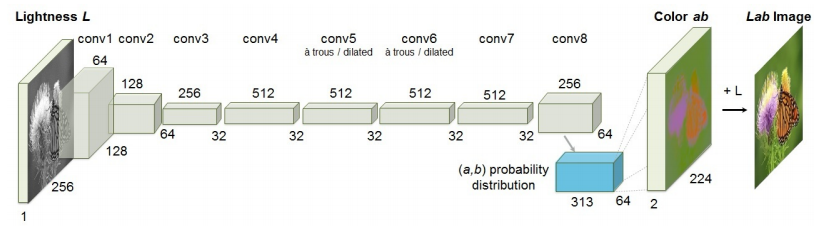
\includegraphics[width=0.7\paperwidth]{color_image_color}
    \caption{Zhang等人的网络结构}
    \label{fig:color_image_color}
  \end{figure}

\section{生成对抗网络}
\label{sec:2-gan}

  生成对抗网络是一种无监督的机器学习模型,最早由Goodfellow~\cite{DBLP:conf/nips/GoodfellowPMXWOCB14}等人在2014年提出,这种模型多用于数据或图像的自动生成,在最近几年里有大量关于GAN的研究,也出现了很多GAN的变体。生成对抗模型的基本结构如图~\ref{fig:gan},其思想为同时训练两个神经网络,一个生成器(generator),一个判别器(discriminator)。输入随机变量到生成器,将期望生成的真实图像与生成器生成的图像混合着输入给判别器,让判别器判断哪些是真实图像哪些是假的图像;通过判别器给出的概率与真实标签的距离更新判别器,同时通过判别器给出的生成器生成图片的真实概率更新生成器。这样两个网络就构成了一种对抗关系,当迭代训练后判别器也难以判断图像的真假,训练好的生成器就可以做图像或数据生成了。

  \begin{figure}[H]
    \centering
    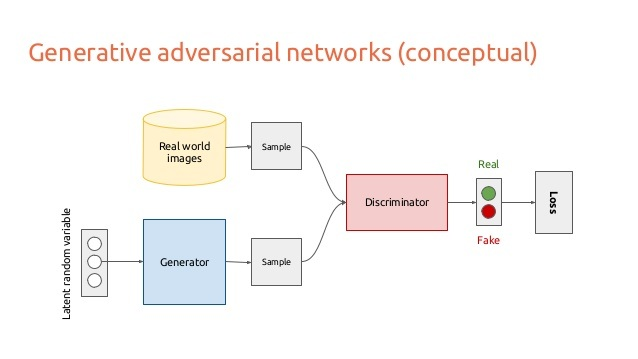
\includegraphics[width=0.7\paperwidth]{gan}
    \caption{生成对抗模型}
    \label{fig:gan}
  \end{figure}

\subsection{cGAN与wGAN}
\label{sec:2-cgan-and-wgan}
  
  GAN模型经过几年的发展出现了许多变体,下面介绍对着色问题有用的带条件的生成对抗网络与沃瑟斯坦生成对抗网络。

  cGAN由Mirza~\cite{DBLP:journals/corr/MirzaO14}等人在2014年提出,基本结构如图~\ref{fig:cgan}。其最重要的一点思想就是当网络需要输入一些额外信息时(例如着色问题中的灰度图像),将这个额外信息同时输入给生成器和判别器,而不是只输入到生成器。实验证明,这样的方式可以让生成器与判别器都收敛得更好。

  \begin{figure}[H]
    \centering
    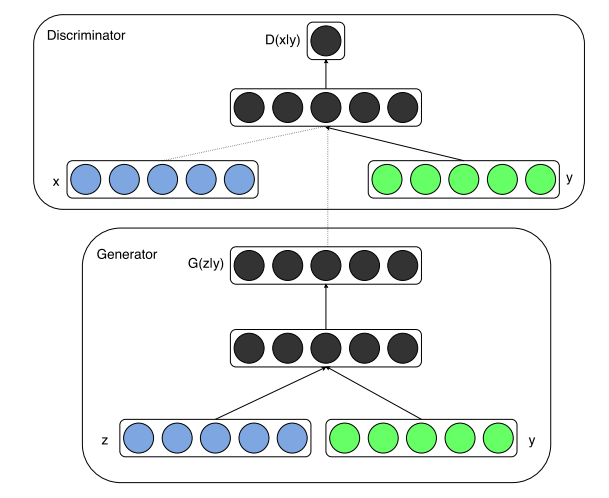
\includegraphics[width=0.7\paperwidth]{cgan}
    \caption[带条件的生成对抗模型]{带条件的生成对抗模型,y即额外信息}
    \label{fig:cgan}
  \end{figure}

  而wGAN的工作则是对原始GAN结构的一些优化,由Arjovsky~\cite{DBLP:journals/corr/ArjovskyCB17}等人2017年提出。我们已经知道GAN是同时训练生成器网络与判别器网络,而且两者的最优化目标是对立的。那么就会有一个平衡二者训练的问题存在:一般情况下,判别器的任务更简单,所以收敛的比生成器就更快,如果判别器早早的就收敛到了很好的状态,生成器怎么更新都无法欺骗判别器,这样生成器的学习就停止了,最后也无法得到好的生成网络。而wGAN就是要解决GAN训练不稳定的问题,他们对原始GAN主要做了4点改动:

  \begin{enumerate}
    \item 判别器最后一层去掉了sigmoid
    \item 生成器以及判别器的损失函数不取对数
    \item 每次更新判别器的参数之后,用一个固定常数将它们的绝对值截断
    \item 不用基于动量的优化算法
  \end{enumerate}

  虽然只是几点小小的改动,Arjovsky~\cite{DBLP:journals/corr/ArjovskyB17}等人在另一篇论文中从数学上证明了这样是可以使GAN稳定训练的,而不需要人工控制生成器与判别器的训练比例。

\subsection{变分自编码器}
\label{sec:2-vae}
  
  对于着色问题而言,我们要通过输入灰色图像得到色度图像输出,而通用的GAN模型中生成器网络的输入是一个噪声向量,所以有必要对生成器网络做一些修改。变分自编码器(VAE)跟GAN一样是非常常用的无监督学习模型,由Kingma~\cite{DBLP:journals/corr/KingmaW13}等人2013年提出。变分自编码器主要由编码器网络与解码器网络组成,如图~\ref{fig:vae}所示,其作用是可以将图片编码为特征向量然后解码出来,为图片变换提供了可能。

  \begin{figure}[H]
    \centering
    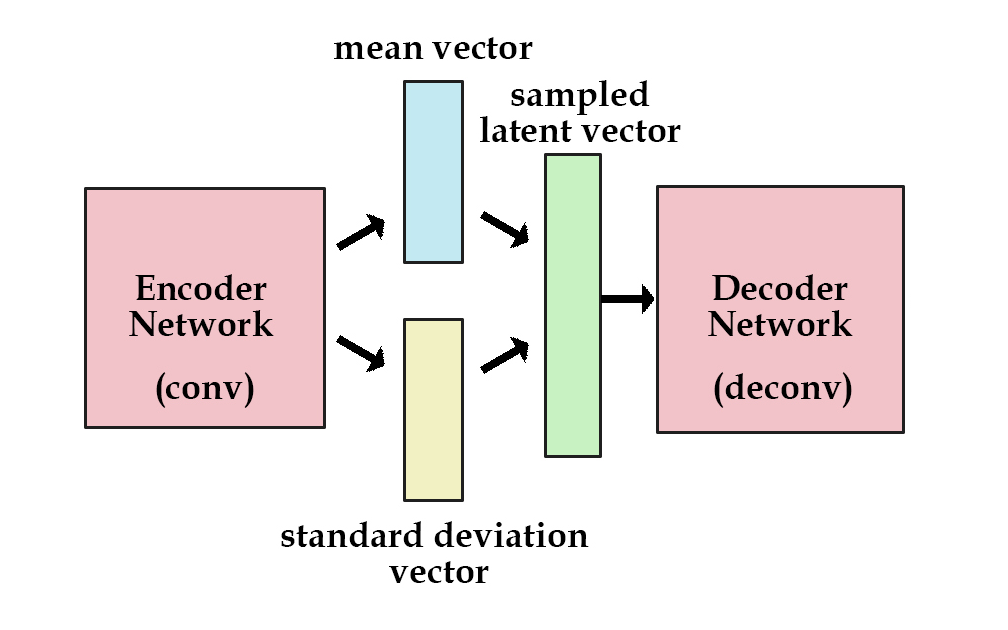
\includegraphics[width=0.7\paperwidth]{vae}
    \caption{变分自编码器}
    \label{fig:vae}
  \end{figure}


\chapter{黑白视频着色算法}
\label{cha:3-video-color}

  本章介绍了本文中使用的所有网络、算法。第\ref{sec:3-image-color}节介绍了本文黑白图像着色的模型选择,经过验证的模型在第\ref{sec:3-video-color}节中应用到了黑白视频着色上。第\ref{sec:3-other-algorithm}节介绍了用于帧内帧间的平滑算法与非关键帧着色算法。最后\ref{sec:3-experiment}节展示了实验结果。

\section{黑白图像着色}
\label{sec:3-image-color}

  基于wGAN的架构,本文训练了几种模型用于黑白图像着色,下面介绍本文的网络结构以及相关训练参数。

\subsection{判别器网络}
\label{sec:3-image-dnet}
  
  判别器网络使用了比较常见的CNN网络,其详细参数如下:对于分辨率为64x64的图像,判别器中有4层卷积层与其对应的BN层和LeakyReLU层,每个卷积核均为4,步幅为2,边缘填充为1。这样每个卷积层都是图像分辨率减半,特征通道数翻倍。在得到4x4的特征后,再经过一个卷积核为4,步幅为1,边缘填充为0的卷积层,就得到输出的1x1的结果,即判别器给出的图像是真实的概率。
  
\subsection{生成器网络}
\label{sec:3-image-gnet}

  生成器网络是GAN中最重要的一部分,因为它的是否合适决定了最终生成器能否生成理想的结果。本文尝试了基线模型,变分自编码器与U-NET几种结构。对于着色问题而言,本文在所有的生成器网络结构中都没有使用池化层,因为池化层是通过压缩空间上的信息来降低分辨率,这样会丢失一些信息,所以本文都是通过步幅大于1的卷积层达到压缩的目的。


  \begin{enumerate}
  \item 基线模型
  
  着色问题与一般分类、回归问题的很大不同在于,着色的输入输出分辨率是一样的,在网络中传递时空间上的信息需要得到很好的保持。于是最初尝试的是一个最简单的网络结构:五个卷积层及其对应的BN层和ReLU层,其中前三个卷积层均核为3,步幅为1,以及1的边缘填充。这样在前三层图像的分辨率都没有变化。后两层卷积层核为1,步幅为1,边缘填充为0,这样在后两层图像分辨率也不发生变化。最后一层卷积层不带BN层与ReLU层。网络结构如图~\ref{fig:fcn}所示。

  \begin{figure}[H]
    \centering
    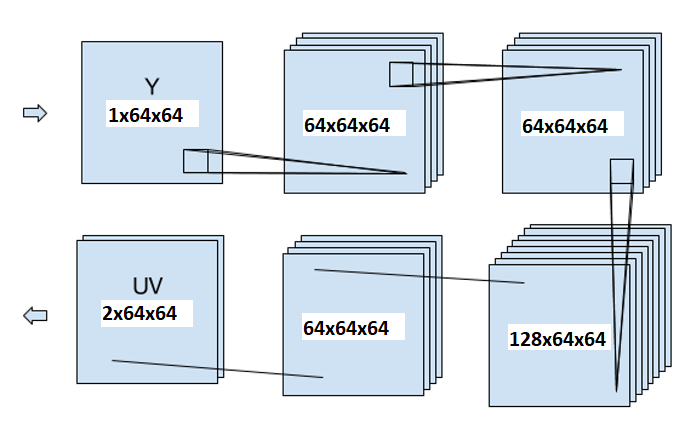
\includegraphics[width=0.5\paperwidth]{fcn}
    \caption{基线模型}
    \label{fig:fcn}
  \end{figure}

  另外一个选择是是网络层的通道数,输入的灰度图像通道为1,输出的色度图像通道为2,中间的卷积层通道数为64或128,翻倍以后再减半回来。通道数的数量在一定程度上代表了网络的最大学习能力,所以在网络使用了较多的特征通道。

  \item 变分自编码器

  变分自编码器的结构在相关工作中已经介绍过了,在本文的网络中做了一些简化,结构如图~\ref{fig:vae-2},称为编码解码模型(encoder-and-decoder)。

  \begin{figure}[H]
    \centering
    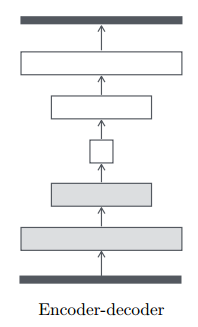
\includegraphics[width=0.2\paperwidth]{vae_2}
    \caption{编码解码模型结构示意}
    \label{fig:vae-2}
  \end{figure}

  该模型与基线模型的一点区别在于,网络卷积中图像分辨率是变化的,是一个先缩小后变大还原,即卷积与反卷积的过程,卷积的部分就是编码器,反卷积的部分就是解码器。编码器会将图像压缩到分辨率为1x1的特征向量,然后解码器将这个特征向量(即GAN模型中的随机变量)映射到色度图像。

  这个模型的详细参数如下:对于分辨率为64x64的图像,编码器包含6层卷积层及其对应的BN层和ReLU层,每个卷积层均核为4,步幅为2,边缘填充为1。每个步幅为2的卷积层都会让图像在空间上减半,特征通道上翻倍(有几个卷积层保持而不翻倍通道数)。这样图像经过编码器后得到1x1x256的特征向量。解码器包含6个反卷积层及其对应的BN层和ReLU层,每个反卷积层均核为4,步幅为2,边缘填充为1。每个步幅为2的反卷积层都会让图像在空间上翻倍,特征通道上减半(与编码器网络对应)。这样解码器输出双通道原始分辨率的图像,最后再经过一个tanh的激活函数,这在图像生成的问题上被证明是很有用的。编码器中的ReLU激活函数是LeakyReLU,而解码器中是ReLU。

  \item U-NET

  U-NET的网络结构与编码解码模型非常类似,不过在编码器与解码器的堆成卷积层(即分辨率)之间添加了捷径,即将编码器卷积层得到的特征信息连接到到解码器对应的卷积层一起输入,如图~\ref{fig:unet}所示,这样的好处是编码器中的特征有助于在解码阶段的空间信息恢复。U-NET的结构由Ronneberger~\cite{DBLP:journals/corr/RonnebergerFB15}等人2015提出,被用于生化领域的图像分割。Isola~\cite{DBLP:journals/corr/IsolaZZE16}等人在pix2pix论文中使用了这种结构,他们的任务是不同图像之间的转换,例如猫的手绘轮廓与猫的图片之间的转换,也是图像生成的范围,去掉了会丢失信息的池化层。所以本文的U-NET结构也是学习了他们的模型。

  \begin{figure}[H]
    \centering
    \subcaptionbox{原始U-NET结构\label{fig:unet_origin}}
      {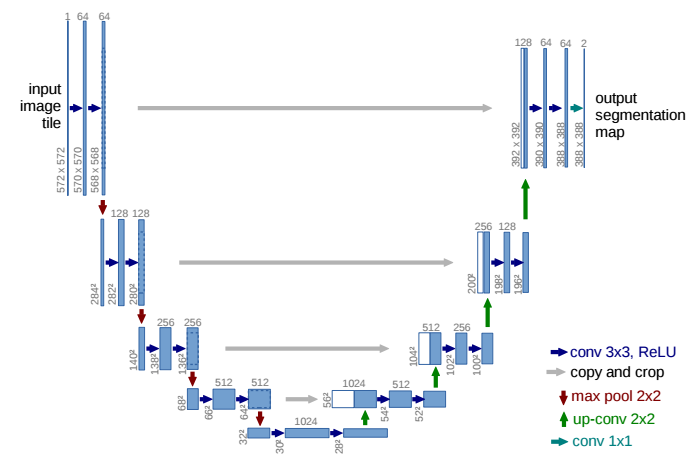
\includegraphics[width=0.45\paperwidth]{unet_origin}}
    \hspace{4em}
    \subcaptionbox{本文的U-NET结构示意\label{fig:unet}}
        {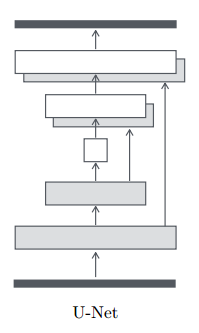
\includegraphics[width=0.15\paperwidth]{unet}}
    \caption{U-NET网络结构}
    \label{fig:unet}
  \end{figure}

  \end{enumerate}

\subsection{训练参数}
\label{sec:3-image-train}

  训练的相关参数如表~\ref{tab:3-image-train}。

  \begin{table}[ht]
    \centering
    \begin{minipage}[t]{0.8\linewidth}
    \caption{黑白图像着色GAN训练参数}
    \label{tab:3-image-train}
      \begin{tabularx}{\linewidth}{lXX}
        \toprule[1.5pt]
        {\heiti 参数名} & {\heiti 描述} & {\heiti 参数值} \\\midrule[1pt]
        image size & 图像分辨率 & 64x64 \\
        batch size & 批处理大小 & 64 \\
        epochs & 重复训练次数 & 200 \\
        ndf & 判别器第一层特征通道数 & 64 \\
        ngf & 生成器第一层特征通道数 & 64 \\
        learn rate D & 判别器学习率 & $5\times10^{-5}$ \\
        learn rate G & 生成器学习率 & $5\times10^{-5}$ \\
        D iterations & 每迭代一次生成器,判别器的迭代次数 & 5 \\
        clamp & 固定判别器参数的常数 & $\pm0.01$ \\
        optimizer & 优化函数 & RMSprop \\
        \bottomrule[1.5pt]
      \end{tabularx}
    \end{minipage}
  \end{table}

  下面对训练参数进行一些解释。图像分辨率使用了较低的64x64,因为图像分辨率增大会使得训练困难以及变慢,所以在初期均使用了较低的分辨率,以达到快速学习,验证模型可行性的目的;D iterations参数的意义是在训练的初期多进行判别器的训练,使得判别器一开始处于一个较准确的状态,从而帮助生成器学习;RMSprop优化函数是深度学习的奠基人之一Geoffrey Hinton~\cite{Tieleman2012}提出的,其目的是解决Adaptive Gradient中学习速率趋向于0的问题。

  另外,我们已经知道生成器的输入是单通道的灰度图像,使用的是YUV色彩空间的Y通道,输出是双通道的色度图像,使用的是YUV中的UV通道,训练图像的YUV值均归一化到[-1,1]。

\section{黑白视频着色}
\label{sec:3-video-color}

  在2D模型上验证了可行性后,就要将模型扩展到3D上处理黑白视频着色问题。本文使用GAN做视频着色的想法来源于3D-GAN的论文~\cite{DBLP:conf/nips/0001ZXFT16}。这篇论文的目的是从一个随机变量生成3D像素空间的模型,有趣的是他们还训练了一个生成器为VAE模型的网络,用于将2D图片转换为3D模型。对于本文的问题而言,从2D扩展到3D不是在空间上,而是在时间上。另外本文并不是将整个视频作为3D数据输入,因为每个视频的长短不一样,网络无法处理帧数不一样的各个视频,所以本文采取等间距采样获取一定数量的关键帧,将这部分关键帧通过网络着色后再用非学习的方法给剩余未着色的帧着色。

  本文的3D着色模型判别器与生成器均分别从2D对应的模型扩展而来,下面介绍本文的网络结构以及训练参数。

\subsection{判别器网络}
\label{sec:3-video-dnet}
  
  判别器网络直接从图片着色网络扩展而来:使用3D的卷积函数和3D的BN函数;之前的卷积核是2D的,大小为4x4,扩展到3D后,大小为4x4x4,同样步幅由2x2变为2x2x2,边缘填充由1x1变为1x1x1。卷积层及其对应的BN层和LeakyReLU层还是4层。最后经过一个卷积核为1x4x4的卷积层得到判别器给出的图像为真实的概率。卷积核大小为1x4x4的原因在第\ref{sec:3-video-train}节解释。
  
\subsection{生成器网络}
\label{sec:3-video-gnet}

  本文的生成器网络选择从U-NET扩展到3D,因为在黑白图像着色阶段被证明U-NET是最好的结构。这个网络的结构如下:输入64x64x8的单通道图像序列,经过6层卷积核4、步幅2、边缘填充1的卷积层及其对应的BN层和LeakyReLU层,得到1x1x1x256的特征向量,然后经过6层卷积核卷积核4、步幅2、边缘填充1的反卷积层,得到64x64x8的双通道图像,再经过一层tanh激励函数后得到输出色度图像序列。其中在解码的反卷积阶段,前面对应的编码卷积层的输出特征都添加到反卷积输入中,以帮助空间信息的恢复。

\subsection{训练参数}
\label{sec:3-video-train}

  黑白视频着色训练的相关参数如表~\ref{tab:4-video-train}。

  \begin{table}[h]
    \centering
    \begin{minipage}[t]{0.8\linewidth}
    \caption{黑白视频着色GAN训练参数}
    \label{tab:4-video-train}
      \begin{tabularx}{\linewidth}{lXX}
        \toprule[1.5pt]
        {\heiti 参数名} & {\heiti 描述} & {\heiti 参数值} \\\midrule[1pt]
        image size & 图像分辨率 & 64x64 \\
        batch size & 批处理大小 & 64 \\
        frame size & 单视频截取帧数 & 8 \\
        epochs & 重复训练次数 & 200 \\
        ndf & 判别器第一层特征通道数 & 64 \\
        ngf & 生成器第一层特征通道数 & 64 \\
        learn rate D & 判别器学习率 & $5\times10^{-5}$ \\
        learn rate G & 生成器学习率 & $5\times10^{-5}$ \\
        D iterations & 每迭代一次生成器,判别器的迭代次数 & 5 \\
        clamp & 固定判别器参数的常数 & $\pm0.01$ \\
        optimizer & 优化函数 & RMSprop \\
        \bottomrule[1.5pt]
      \end{tabularx}
    \end{minipage}
  \end{table}

  视频着色与图像着色的差别就是多了一个单视频截取帧数的参数,在这里本文取值为8,即对于训练数据集中的每个视频,等间距的取出8帧图像代表这个视频,输入给着色网络。帧数上的分辨率小于图像空间上的分辨率就会导致一个问题,即使用卷积核为4的卷积时,帧数维度会先于空间维度压缩到大小为1,继续卷积会出现问题,所以在帧数维度压缩到1后,在帧数维度上的卷积层,设置为卷积核为3,步幅为1,边缘填充为1,这样可以保持帧数维度上1的分辨率不变。这也是本文在判别器最后一层卷积层使用了1x4x4的卷积核的原因。

\section{关键帧平滑与非关键帧着色}
\label{sec:3-other-algorithm}

  在这一节中,将介绍本文用于对着色后的关键帧在空间和时间上平滑的算法,以及得到关键帧平滑着色后用于给非关键帧着色的算法。

  由于一些原因,本文最后的视频着色并没有使用第~\ref{sec:3-video-color}节中的3D模型,而使用的第~\ref{sec:3-image-color}中的2D着色模型,本文将在第~\ref{sec:3-experiment}节中给出解释。

  所以整体算法的流程如下:

  \begin{enumerate}
    \item 对于输入黑白视频,等间距提取出关键帧;
    \item 用训练好的二维GAN网络的生成器网络给关键帧着色;
    \item 分别对每一个关键帧做空间平滑处理;
    \item 综合所有关键帧,依次对其做时间平滑处理;
    \item 利用得到的关键帧颜色对非关键帧进行着色;
    \item 输出着色后的视频。
  \end{enumerate}

\subsection{空间平滑算法}
\label{sec:3-spatial-smooth}

  对于一张黑白图像而言,现在的基于学习的自动着色算法输出的着色或多或少都会存在一些空间上的不连续,很容易被人识别出来,所以需要做一个空间平滑的处理。

  本文的空间平滑算法具体如下:输入待平滑彩色图像,遍历其所有像素;对于每个像素,搜索其邻近的像素(在实验中本文取的以该像素为中心的5x5的patch),如果邻近像素的灰度值与该像素的灰度值差在一定范围内(YUV色彩空间中的Y值),则邻近像素视为与原像素属于同物体;搜索完邻近像素后,将所有被视为原像素同物体的像素的色度值取平均值(YUV色彩空间中的UV值),作为该像素新的色度值。

  算法伪代码如下。

  \begin{algorithm}[H]
  \label{algo:5-spatial-smooth}
    \caption*{空间平滑算法}
    \begin{algorithmic}[1]
      \Require $Y$, $UV$
      \Ensure  $UV$
      \Function{spatial smooth}{}
        \For {pixel $p \in Y$}
          \State $\Omega = \phi$
          \For {pixel $\|p^{'} - p\| <= 2$}
            \If {$\|Y(p) - Y(p^{'})\| < \epsilon$}
              \State $\Omega = \Omega \cup p^{'}$
            \EndIf
          \EndFor
          \State $UV(p) = mean(UV(\Omega))$
        \EndFor
      \EndFunction
    \end{algorithmic}
  \end{algorithm}


\subsection{时间平滑算法}
\label{sec:3-temporal-smooth}

  将关键帧依次给着色网络着色病不能保证视频颜色在时间上的稳定性,这一点本文在第~\ref{sec:3-experiment}节中进行了实验。所以在得到每个关键帧的独立着色后,需要对这一系列关键帧的颜色进行平滑,使它们保持一致性。关键帧的稳定是非关键着色稳定的前提,也是视频颜色稳定的前提。

  本文的时间平滑算法如下:输入一系列按时间排序的关键帧彩色图像,设有K帧,对于每个关键帧,做如下处理:用Gunnar~\cite{DBLP:conf/scia/Farneback03}等人2003年提出的光流算法计算关键帧F其与其他$(K-1)$个关键帧之间的光流,这样对关键帧$F$中的每个像素$p$而言,可以找到其在其他关键帧中的$(K-1)$个对应像素,去掉不在图像范围内的,去掉像素灰度值与像素$p$灰度值的差超过一定值的像素,取剩下符合要求像素的色度平均值,作为像素$p$平滑后的色度值。这样对于每个关键帧的每个像素,它们的色度都是比较相近的,排除了着色网络在某些帧会给出与一般情况差别较大的误差。

  算法伪代码如下。

  \begin{algorithm}[H]
  \label{algo:5-temporal-smooth}
    \caption*{时间平滑算法}
    \begin{algorithmic}[1]
      \Require $Ys$, $UVs$
      \Ensure  $UVs$
      \Function{temporal smooth}{}
        \For {$Y_i \in Ys$}
          \For {$Y_j \in Ys$}
            \State $flow = \textbf{GunnarOpticalFlow}(Y_i, Y_j)$
            \For {$p \in Y_i$}
              \State $p^{'} = p + flow(p)$
              \If {$\|Y_i(p) - Y_j(p^{'})\| < \epsilon$}
                \State $\Omega_p = \Omega_p \cup UV_j(p^{'})$
              \EndIf
            \EndFor
          \EndFor
          \For {$p \in Y_i$}
            \State $UV_i(p) = mean(\Omega_p)$
          \EndFor
        \EndFor
      \EndFunction
    \end{algorithmic}
  \end{algorithm}

\subsection{非关键帧着色算法}
\label{sec:3-interframe-color}

  在得到所有关键帧的平滑着色后,就要将关键帧的色度传递到剩余非关键帧。本文的算法采取相邻帧迭代传递色度的方法,即从已着色的关键帧$F_{nk}$开始,用它的颜色传递到它的下一帧$F_{nk+1}$(非关键帧);当第$F_{nk+1}$帧着色完成时,它又可以作为第$F_{nk+2}$帧的参考帧,将颜色传递给第$F_{nk+2}$帧;重复这个过程,当着色到下一个关键帧$F_{n(k+1)}$时,又可以从这个关键帧开始下一轮颜色传递。

  本文的色彩传递算法具体如下:设前一帧参考帧为$F_p$,待着色的帧为$F_c$,首先计算两帧之间的光流,对于$F_c$中的待着色像素$p_c$而言,在$F_p$中可找到光流对应的像素$p_c^{'}$,另外还有$F_p$中与像素$p_c$同位置的$p_p$,取$p_p$周围3x3的patch的像素$N(p_p)$,然后在像素集合${p_c^{'},N(p_p)}$中找与像素$p_c$灰度值差最小的像素$r$,即

  \begin{equation}
  \label{equ:5-interframe}
    r = \mathop{\arg\min}_{p \in \{p_c^{'},N(p_p)\}} \|Y_c(p_c) - Y_p(p)\|^2
  \end{equation}

  然后取$r$的色度值作为$p_c$的色度值。对$F_c$中的每个像素做如上操作即可完成帧$F_c$的着色。

  算法伪代码如下。

  \begin{algorithm}[H]
  \label{algo:5-interframe}
    \caption*{非关键帧着色算法}
    \begin{algorithmic}[1]
      \Require $Y_c$, $Y_p$, $UV_p$
      \Ensure  $UV_c$
      \Function{color flow}{}
        \State $flow = \textbf{GunnarOpticalFlow}(Y_c, Y_p)$
        \For {$p_c \in Y_c$}
          \State $p_c^{'} = p_c + flow(p_c)$
          \State $\Omega = \{p_c^{'}\}$
          \For {$\|p - p_c\| < \epsilon$}
            \State $\Omega = \Omega \cup p$
          \EndFor
          \For {$p \in \Omega$}
            \If {$\|Y_p(p) - Y_c(p_c)\| < min$}
              \State $r = p$
            \EndIf
          \EndFor
          \State $UV_c(p_c) = UV_p(r)$
        \EndFor
      \EndFunction
    \end{algorithmic}
  \end{algorithm}

\section{实验及结果}
\label{sec:3-experiment}
  
  实验对比一节依然分为图像着色与视频着色分别讨论。

\subsection{黑白图像着色}
\label{sec:3-image-color-exp}

  对于图像着色,本文在三个数据集上进行了实验,与两种目前效果最好的学习算法进行了对比。

  三个数据集分别是:LSUN-CHURCH~\cite{DBLP:journals/corr/YuZSSX15},是一个教堂图片的数据集,数据规模为12w训练集,300验证集;CIFAR-10~\cite{CIFAR-10},是一个包含10类图片的数据集,数据规模为5w训练集,1w测试集;IMAGE-NET~\cite{DBLP:journals/ijcv/RussakovskyDSKS15},是一个大型的分类数据集,包含1000类物体,本文采用了它的部分子集,数据规模为28w训练集,1w测试集。

  进行对比的两个图像自动着色算法是Iizuka等人Siggraph2016的\inlinecite{IizukaSIGGRAPH2016},与Zhang等人ECCV2016的\inlinecite{zhang2016colorful}。

  本文选择均方误差(MSE)作为评价标准,即以网络着色结果与真是彩色图像之间的像素均方差作为误差。表~\ref{tab:6-image-error}给出了误差对比。需要注意的是,本文的网络是在三个数据集下分别独立的,即Ours$_l$指的是在LSUN-CHURCH下训练的本文的网络,Ours$_c$与Ours$_i$以此类推;另外,均方误差值取的是64x64分辨率图片的像素误差和,且像素UV值已归一化到[-1,1]。

  \begin{table}[H]
    \centering
    \begin{minipage}[t]{0.8\linewidth}
    \caption{黑白图像着色均方误差对比}
    \label{tab:6-image-error}
      \begin{tabularx}{\linewidth}{|l|X|X|X|}
        \hline
        \multirow{2}*{\diagbox[width=6em]{\heiti 方法}{\heiti 数据集}} & \multirow{2}*{LSUN-CHURCH} & \multirow{2}*{CIFAR-10} & \multirow{2}*{IMAGE-NET} \\
         & & & \\\hline
        Ours$_l$ & 127.1 & - & - \\\hline
        Ours$_c$ & - & 347.9 & - \\\hline
        Ours$_i$ & - & - & 174.5 \\\hline
        Zhang    & 151.8 & 367.5 & 282.8 \\\hline
        Iizuka   & \textbf{86.7}  & \textbf{117.2} & \textbf{127.6} \\\hline
      \end{tabularx}
    \end{minipage}
  \end{table}

  从表~\ref{tab:6-image-error}进行方法的纵向对比,可以发现本文的生成对抗模型总体来说表现比Zhang~\cite{zhang2016colorful}等人的卷积神经网络好,但与Iizuka~\cite{IizukaSIGGRAPH2016}等人的卷积神经网络相比还差距较大;在本文的方法内部进行数据集间的横向对比可以发现:当在只有一类物体的LSUN-CHURCH数据集上时,本文的均方误差较小,当在物体种类较多的IMAGE-NET上训练时,误差变大;当图像分辨率变小时(CIFAR-10的图像分辨率只有32x32),误差也会明显增大。

  图~\ref{fig:lsun-compare},图~\ref{fig:cifar-compare},图~\ref{fig:imagenet-compare}分别给出了LSUN-CHURCH、CIFAR-10、IMAGE-NET数据集下本文的网络着色与真实图像的对比。

  \begin{figure}[ht]
    \centering
    \subcaptionbox{本文网络的着色结果\label{fig:lsun_fake}}
      {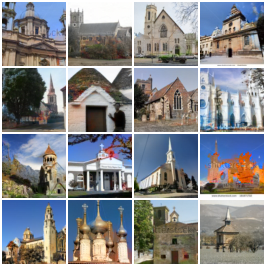
\includegraphics[width=0.3\paperwidth]{lsun_fake}}
    \hspace{2em}
    \subcaptionbox{真实彩色图像\label{fig:lsun_real}}
        {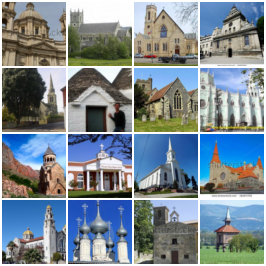
\includegraphics[width=0.3\paperwidth]{lsun_real}}
    \caption{LSUN-CHURCH数据集测试结果}
    \label{fig:lsun-compare}
  \end{figure}

  \begin{figure}[ht]
    \centering
    \subcaptionbox{本文网络的着色结果\label{fig:cifar_fake}}
      {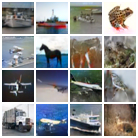
\includegraphics[width=0.3\paperwidth]{cifar_fake}}
    \hspace{2em}
    \subcaptionbox{真实彩色图像\label{fig:cifar_real}}
        {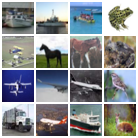
\includegraphics[width=0.3\paperwidth]{cifar_real}}
    \caption{CIFAR-10数据集测试结果}
    \label{fig:cifar-compare}
  \end{figure}

  \begin{figure}[ht]
    \centering
    \subcaptionbox{本文网络的着色结果\label{fig:imagenet_fake}}
      {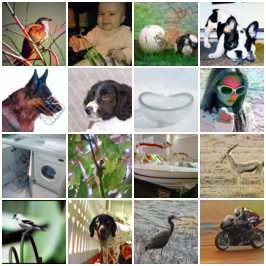
\includegraphics[width=0.3\paperwidth]{imagenet_fake}}
    \hspace{2em}
    \subcaptionbox{真实彩色图像\label{fig:imagenet_real}}
        {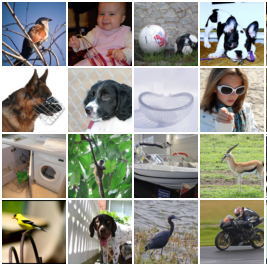
\includegraphics[width=0.3\paperwidth]{imagenet_real}}
    \caption{IMAGE-NET数据集测试结果}
    \label{fig:imagenet-compare}
  \end{figure}

  从这些结果中分析得出这样的结论:GAN处理着色问题相比CNN更逊色。图像风格转换的任务已经被证明非常适合GAN模型,Zhu~\cite{DBLP:journals/corr/ZhuPIE17}等人最新的网络结构cycleGAN在做两种风格图片转换的任务上取得了很好的效果,比如油画风格与照片写实风格之间的互相转换。着色问题也可以看作一个风格转换问题(黑白风格到彩色风格的转换),但相比前者,着色问题里图像的域更大:前者可能只是莫奈的油画风格与真实照片的转换,而着色中的图像包含了多种物体的多种可能颜色,对于一种物体有效的着色对于另一种物体就不行。所以在单一物体的LSUN-CHURCH数据集上表现更好,而在多物体的CIFAR-10与IMAGE-NET的数据集上就表现更差。

\subsection{黑白视频着色}
\label{sec:3-video-color-exp}

  对于视频着色,本文在UCF11数据集上进行了实验,与之前的最先进的自动黑边图像着色算法直接应用于视频进行了对比。

  UCF11~\cite{DBLP:conf/cvpr/LiuLS09}是一个人体动作识别的数据库,包含11类人类不同运动的短视频共2000段。在这个数据集上使用本文第~\ref{sec:3-video-color}节中的3D模型时,生成器无法向真实图像进行学习,结果是着色的关键帧一直是非常暗淡没有什么色彩,在反复调试后也不能得到有意义的结果,图~\ref{fig:3d_result}就是本文的3D网络着色结果。于是只好暂时放弃用3D模型着色的想法,使用2D的GAN模型给关键帧着色。

  \begin{figure}[H]
    \centering
    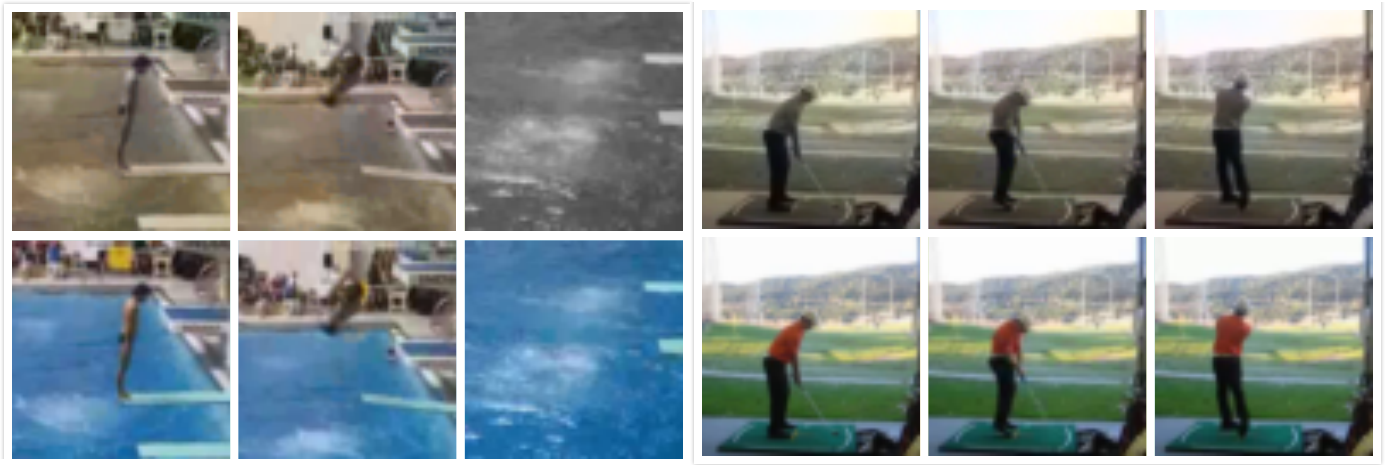
\includegraphics[width=0.7\paperwidth]{3d_result}
    \caption[3D网络着色结果]{3D网络的着色结果。第一行是本文的着色,第二行是真实视频帧;前三列来自一个跳水视频,后三列来自一个高尔夫视频}
    \label{fig:3d_result}
  \end{figure}

  使用2D网络对视频着色的流程在第~\ref{sec:3-other-algorithm}节已经介绍过了。训练时本文使用UCF11中的2000个视频,每个视频等间距取采样帧作为训练图像数据,共约2w的训练集,测试集有约100个独立的视频。

  图~\ref{fig:2d_result}是本文的2D网络着色结果。

  \begin{figure}[H]
    \centering
    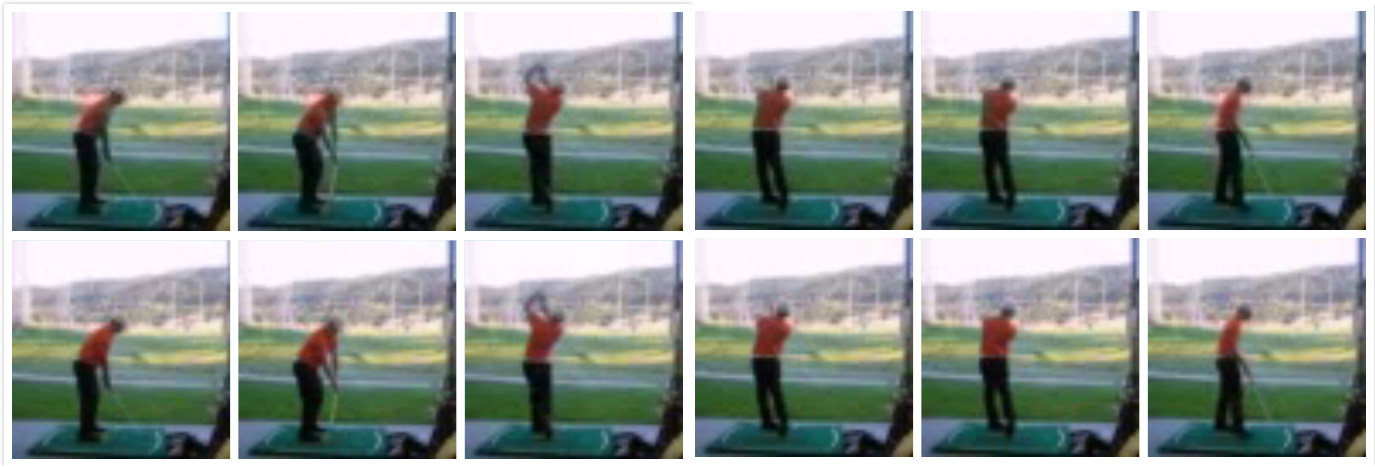
\includegraphics[width=0.7\paperwidth]{2d_result}
    \caption[2D网络着色结果]{3D网络的着色结果。第一行是我们的着色视频帧,第二行是真实视频帧}
    \label{fig:2d_result}
  \end{figure}

  另外单帧着色带来的时间空间不稳定性通过本文第~\ref{sec:3-other-algorithm}节中的平滑可以解决,这一点可以从图~\ref{fig:2d_result_compare}中看出。

  \begin{figure}[H]
    \centering
    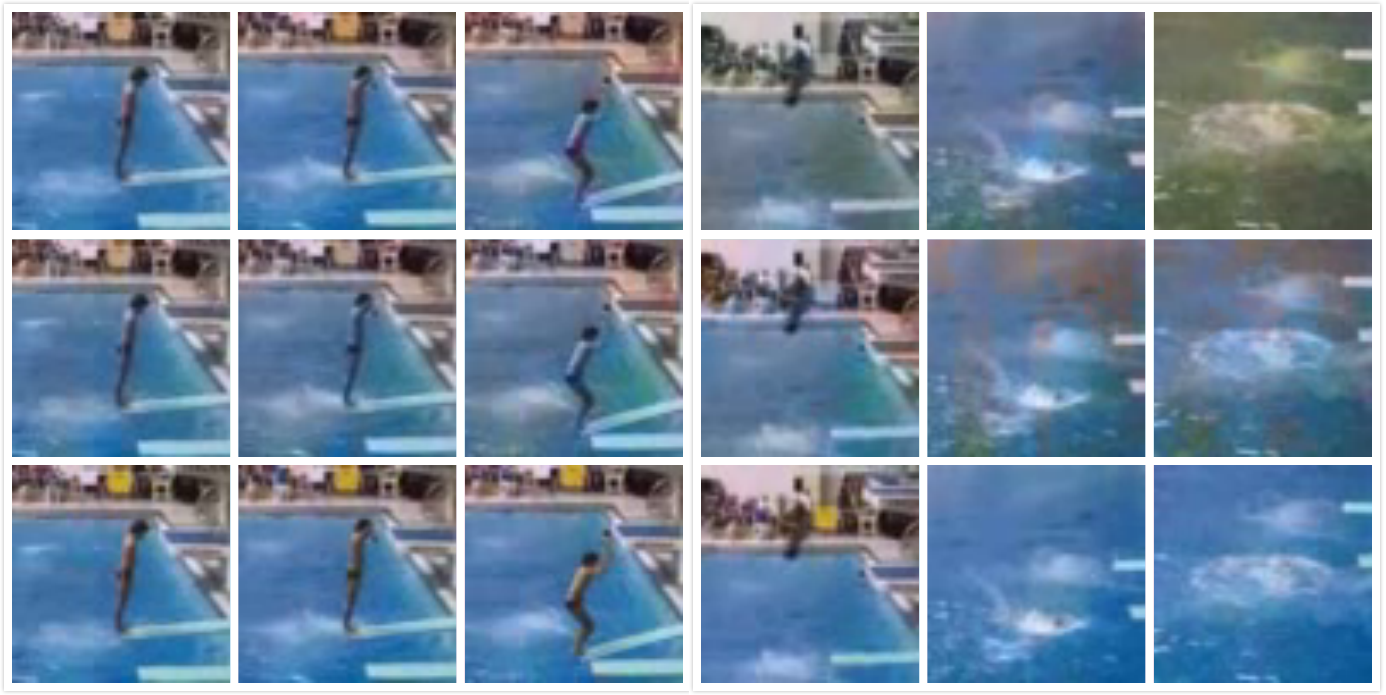
\includegraphics[width=0.7\paperwidth]{2d_result_compare}
    \caption[时空平滑效果比较]{时空平滑效果比较。第一行是本文直接使用2D网络对每一帧着色的结果,第二行是本文用2D网络对关键帧着色然后进行时空平滑处理的结果,第三行是真实视频帧}
    \label{fig:2d_result_compare}
  \end{figure}

  表\ref{tab:3-video-error}给出了我们的方法与Iizuka和Zhang方法的量化对比。在着色准确度方面,我们计算了测试视频与真实视频每帧像素之间的均方误差;在时间一致性方面,我们计算了测试视频着色结果每对相邻帧之间的均方误差。可以看到,我们的着色准确度相比另外两个方法要好,而时间一致性方面,Iizuka方法的误差最小,甚至比真实视频的误差还低,经验证发现Iizuka方法对视频的着色效果不太好,着色后的视频与初始的灰度视频差不多,所以在时间连续性误差上较小。综合两项,本文的方法在UCF11视频数据集上表现比其他两个方法要好。

  \begin{table}[H]
    \centering
    \begin{minipage}[t]{0.8\linewidth}
    \caption{黑白视频着色误差对比}
    \label{tab:3-video-error}
      \begin{tabularx}{\linewidth}{|l|X|X|}
        \hline
        \multirow{2}*{\diagbox[width=8em]{\heiti 方法}{\heiti 评测方法}} & \multirow{2}*{均方误差} & \multirow{2}*{时间连续性误差} \\
         & & \\\hline
        Ground Truth & 0 & 2.55 \\\hline
        Ours & \textbf{161.01} & 6.14 \\\hline
        Zhang & 757.75 & 26.03 \\\hline
        Iizuka & 499.17 & \textbf{1.59} \\\hline
      \end{tabularx}
    \end{minipage}
  \end{table}

  另外本文也用图像着色中LSUN-CHURCH教堂数据集训练的网络给大礼堂进行了着色,如图~\ref{fig:extra_result}。

  \begin{figure}[H]
    \centering
    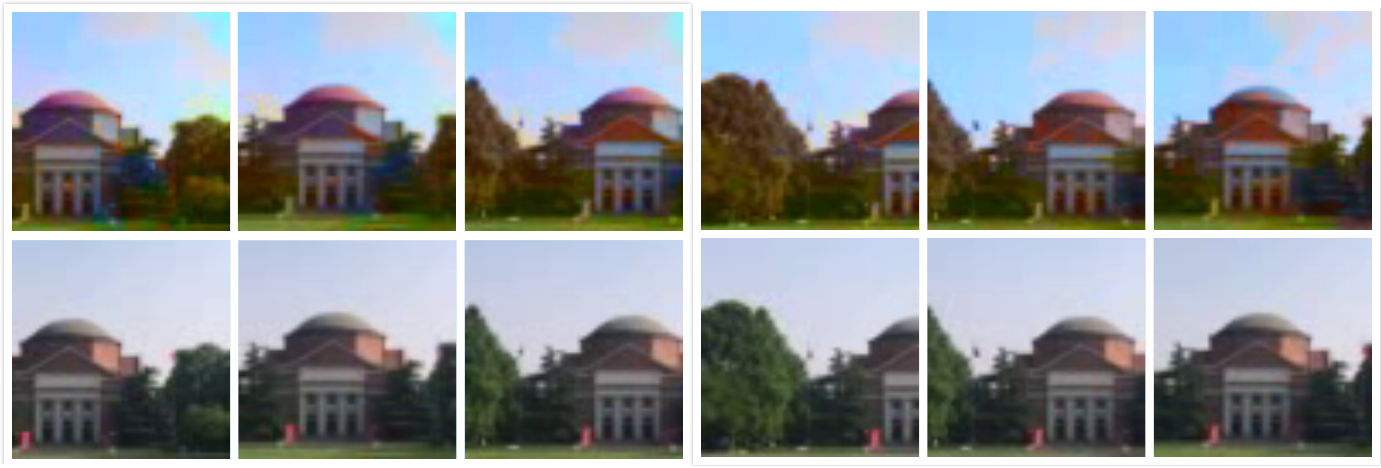
\includegraphics[width=0.7\paperwidth]{extra_result}
    \caption[大礼堂着色效果]{大礼堂着色效果。第一行是本文的着色结果,第二是真实拍摄的视频}
    \label{fig:extra_result}
  \end{figure}

  \begin{figure}[H]
    \centering
    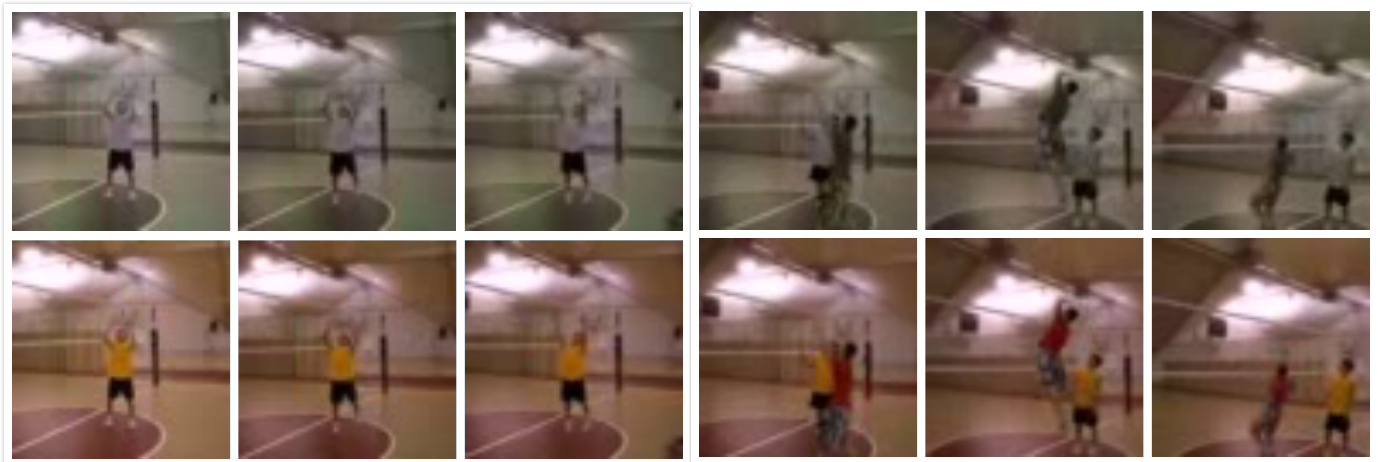
\includegraphics[width=0.7\paperwidth]{failure_case}
    \caption[失败案例]{失败案例。第一行是本文的着色结果,第二是真实拍摄的视频}
    \label{fig:failure_case}
  \end{figure}  

  不过在UCF11数据集下也有一些失败的案例,如图~\ref{fig:failure_case},通常的体现是没有什么色彩。分析原因为:当视频场景中物体动作幅度不是很大时,着色能有较好的效果(如高尔夫击球),相反动作幅度较大时(如排球扣球),网络便不那么稳定;场景的特征颜色较明显时(如跳水中的蓝色),着色结果很理想,而场景没有明显的颜色特征时,网络变只能给出灰褐色的平凡结果。





  
\chapter{黑白视频着色}
\label{cha:4-video-color}

  在2D模型上验证了可行性后,就要将模型扩展到3D上处理黑白视频着色问题。本文使用GAN做视频着色的想法来源于3D-GAN的论文~\cite{DBLP:conf/nips/0001ZXFT16}。这篇论文的目的是从一个随机变量生成3D像素空间的模型,有趣的是他们还训练了一个生成器为VAE模型的网络,用于将2D图片转换为3D模型。对于本文的问题而言,从2D扩展到3D不是在空间上,而是在时间上。另外本文并不是将整个视频作为3D数据输入,因为每个视频的长短不一样,网络无法处理帧数不一样的各个视频,所以本文采取等间距采样获取一定数量的关键帧,将这部分关键帧通过网络着色后再用非学习的方法给剩余未着色的帧着色。

  本文的3D着色模型判别器与生成器均分别从2D对应的模型扩展而来,下面介绍本文的网络结构以及训练参数。

\section{判别器网络}
\label{sec:4-d-net}
  
  判别器网络直接从图片着色网络扩展而来:使用3D的卷积函数和3D的BN函数;之前的卷积核是2D的,大小为4x4,扩展到3D后,大小为4x4x4,同样步幅由2x2变为2x2x2,边缘填充由1x1变为1x1x1。卷积层及其对应的BN层和LeakyReLU层还是4层。最后经过一个卷积核为1x4x4\footnote{卷积核大小为1x4x4的原因在第\ref{sec:4-train}节解释}的卷积层得到判别器给出的图像为真实的概率。
  
\section{生成器网络}
\label{sec:4-g-net}

  本文的生成器网络选择从U-NET扩展到3D,因为在黑白图像着色阶段被证明U-NET是最好的结构。这个网络的结构如下:输入64x64x8的单通道图像序列,经过6层卷积核4、步幅2、边缘填充1的卷积层及其对应的BN层和LeakyReLU层,得到1x1x1x256的特征向量,然后经过6层卷积核卷积核4、步幅2、边缘填充1的反卷积层,得到64x64x8的双通道图像,再经过一层tanh激励函数后得到输出色度图像序列。其中在解码的反卷积阶段,前面对应的编码卷积层的输出特征都添加到反卷积输入中,以帮助空间信息的恢复。

\section{训练参数}
\label{sec:4-train}

  黑白视频着色训练的相关参数如表~\ref{tab:4-video-train}。

  \begin{table}[h]
    \centering
    \begin{minipage}[t]{0.8\linewidth}
    \caption{黑白视频着色GAN训练参数}
    \label{tab:4-video-train}
      \begin{tabularx}{\linewidth}{lXX}
        \toprule[1.5pt]
        {\heiti 参数名} & {\heiti 描述} & {\heiti 参数值} \\\midrule[1pt]
        image size & 图像分辨率 & 64x64 \\
        batch size & 批处理大小 & 64 \\
        frame size & 单视频截取帧数 & 8 \\
        epochs & 重复训练次数 & 200 \\
        ndf & 判别器第一层特征通道数 & 64 \\
        ngf & 生成器第一层特征通道数 & 64 \\
        learn rate D & 判别器学习率 & $5\times10^{-5}$ \\
        learn rate G & 生成器学习率 & $5\times10^{-5}$ \\
        D iterations & 每迭代一次生成器,判别器的迭代次数 & 5 \\
        clamp & 固定判别器参数的常数 & $\pm0.01$ \\
        optimizer & 优化函数 & RMSprop \\
        \bottomrule[1.5pt]
      \end{tabularx}
    \end{minipage}
  \end{table}

  视频着色与图像着色的差别就是多了一个单视频截取帧数的参数,在这里本文取值为8,即对于训练数据集中的每个视频,等间距的取出8帧图像代表这个视频,输入给着色网络。帧数上的分辨率小于图像空间上的分辨率就会导致一个问题,即使用卷积核为4的卷积时,帧数维度会先于空间维度压缩到大小为1,继续卷积会出现问题,所以在帧数维度压缩到1后,在帧数维度上的卷积层,设置为卷积核为3,步幅为1,边缘填充为1,这样可以保持帧数维度上1的分辨率不变。这也是本文在判别器最后一层卷积层使用了1x4x4的卷积核的原因。
\chapter{关键帧平滑与非关键帧着色}
\label{cha:5-other-algorithm}

  在这一章中,我们将介绍我们用于对着色后的关键帧在空间和时间上平滑的算法,以及得到关键帧平滑着色后用于给非关键帧着色的算法。

\section{关键帧平滑算法}
\label{sec:5-keyframe-smooth}

  由于一些原因,我们最后的视频着色并没有使用第~\ref{cha:4-video-color}章中的3D模型,而使用的第~\ref{cha:3-image-color}中的2D着色模型,我们将在~\ref{cha:6-experiment}中给出解释。

  所以我们整体算法的流程是

\subsection{空间平滑算法}
\label{sec:5-spatial-smooth}

\subsection{时间平滑算法}
\label{sec:5-temporal-smooth}

\section{非关键帧着色算法}
\label{sec:5-interframe-color}



%%% 其它部分
\backmatter

%% 本科生要这几个索引,研究生不要。选择性留下。
% 插图索引
\listoffigures
% 表格索引
\listoftables
% 公式索引
\listofequations


%% 参考文献
% 注意:至少需要引用一篇参考文献,否则下面两行可能引起编译错误。
% 如果不需要参考文献,请将下面两行删除或注释掉。
\bibliographystyle{thuthesis}
\bibliography{ref/refs}


%% 致谢
%% 如果使用声明扫描页,将可选参数指定为扫描后的 PDF 文件名,例如:
\begin{acknowledgement}[scan-statement.pdf]
%\begin{acknowledgement}
  由衷的感谢导师王斌教授在毕业设计中给予我的指导。王斌教授在我的选题阶段就给我指明了方向,在后面的研究过程中也是他不断地督促我,帮助我解决问题以及指明下一步的计划。最终毕业设计的完成,离不开王斌老师的指导。

  感谢渲染组的师兄师姐们,他们在每周的组会上帮助我思考解决现有问题的办法,为我提供了很大的帮助。

  感谢三字班的同学们,有他们的帮助我才能顺利完成这次毕业设计,许多困难的时候因为有大家一起帮助才能渡过。

  感谢 \thuthesis,它让我的论文撰写简单了许多,排版变得很轻松。

  最后感谢我的家人,他们在我毕设的过程中提供了我支持与理解,让我能专心完成毕业设计。
\end{acknowledgement}


%% 附录
%\begin{appendix}
%\chapter{外文资料翻译}
\label{cha:engorg}

\renewcommand\thesection{\arabic {section}}

\title{彩色图像着色}

{\heiti 摘要:} 给定一张灰度照片作为输入,本文尝试解决的是给照片上一个合理版本颜色的问题。这个问题明显是不受约束的,所以以前的方法十分依赖于用户交互或者着色结果非常低饱和。我们提出了一个能制造逼真着色结果的全自动的方法。我们将这个问题看成一个分类任务,并且在训练时使用了类别重新平衡方法,从而增加了着色结果中的颜色多样性, 进而解决了颜色不确定的基本问题。我们的系统测试时是一个前向传播的CNN,训练集超过一百万张彩色图像。我们的测试方法是“色彩图灵测试”,要求人类参与者在一张着色生成的照片和真实照片中选择。我们的方法在32\%的实验中成功的欺骗了人类,显著高于以前的方法。此外,我们发现着色作为交叉信道编码器,对于自监督特征学习是一个强大的上游任务。这个方法在几个特征学习的基准测试中都达到最先进的水平。


\section{介绍}
考虑图1中的灰度照片。第一眼看上去,想象他们的颜色对于人类似乎是个很难的任务,因为许多信息(三维中的两维)已经丢失。然而,当更仔细地看,我们可以注意到在许多情况下,场景的语义信息及其表面纹理对于图像中许多区域提供了充足的线索:草通常是绿色的,天空是通常是蓝色的,瓢虫最可能是红色的。当然,这种语义先验并不适用于一切,例如,草地上的槌球现实中可能不是红色,黄色和紫色的(虽然这是一个很好的猜测)。然而,对于本文,我们的目标不一定是恢复实际的真实色彩,而是产生一个合理的结果以至于可以骗过一个人类观察者。因此,我们的任务变得更加可行:只要通过足够的数据在语义信息以及灰度照片的纹理和它们的彩色版本间建模就可以制造出视觉上令人信服的结果。

\begin{figure}[h]
  \centering
  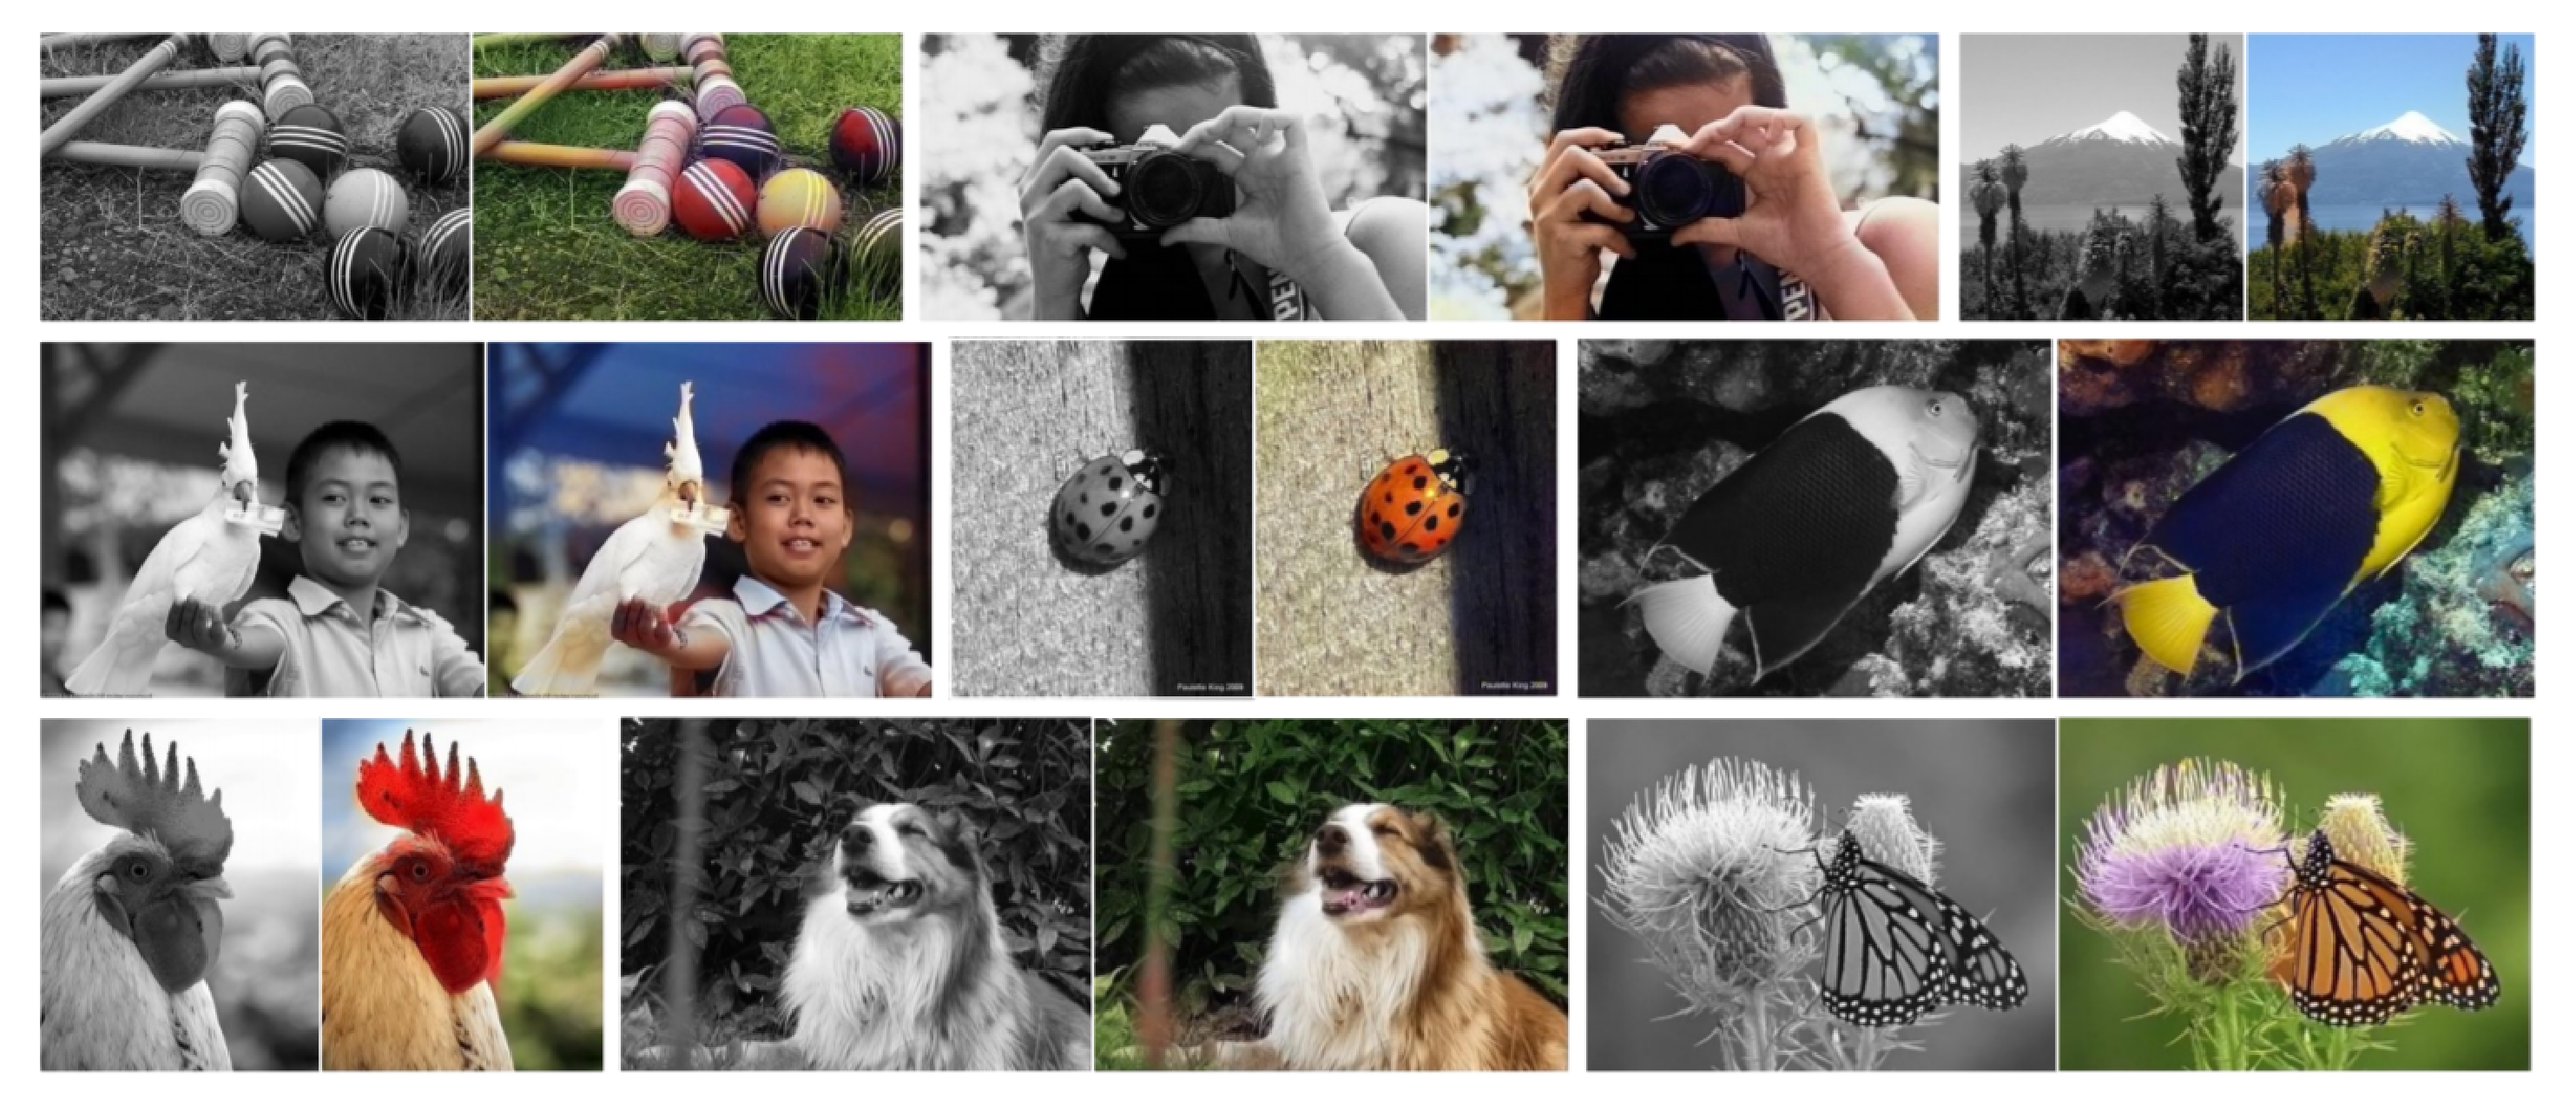
\includegraphics[width=0.7\paperwidth]{appendixF1}
  \caption*{图~1\quad 输入的灰度图像和通过我们的算法输出的彩色结果的样例。这些是选出来的非常好的结果。如果想看所有的结果或者尝试我们的模型和代码,请访问\url{http://richzhang.github.io/colorization/}}
  \label{tab:badfigure1}
\end{figure}

给定亮度通道L,我们的系统在CIE Lab颜色空间预测图像对应的a和b颜色通道。为了解决这个问题,我们利用了大数据。 预测颜色有一点很好的属性就是训练数据是免费可得的:任何彩色照片都可以用作训练样本,简单的通过将图像的L通道作为输入以及其ab通道作为标定结果。 有人也注意到训练数据的易得性,并且之前的工作已经训练了卷积神经网络(CNN)用来预测大数据集上的颜色。 然而,之前工作的结果倾向于看起来不饱和。 一个解释是他们使用了鼓励保守预测的损失函数。 这些偏差来源于标准回归问题,而标准回归问题的目标是在预测结果和真实值之间最小化欧氏距离。

相反我们使用了针对着色问题的损失函数。 正如中指出的,颜色预测本质上是多模式的 - 许多物体可以有好几种可能的合理着色。 例如,苹果通常是红色,绿色或黄色的,但不可能是蓝色或橙色。为了给这个多模态问题适当地建模 ,我们对每个像素预测了可能颜色的分布。此外,为了强调稀有的颜色,在训练时我们重新调整了损失。这鼓励我们的模型在训练集上探索大量数据的全面多样性。 最后,我们通过在颜色分布上取退火平均值的方法产生最终的着色结果。 最终的结果相比之前的方法就有更加生动的色彩并且视觉上更逼真。

评估合成的图像是一个众所周知的难题。 因为我们的终极目标是使结果令观察者信服,我们引入了一种新颖的评估着色结果的方法——直接测试它们的现实真实感。 我们建立了一个“色彩图灵测试”,在测试中展示给参与者一张真实图像和这张图像的机器着色版本,要求他们识别出假的图像。在这个相当困难的标准中,我们能够在32\%实例(两张都是真实照片的话概率将是50\%)中欺骗参与者,显著高于以前的工作。 这个测试表明,在许多情况下,我们的算法都产生近似逼真的结果(参见图1的经过挑选的我们算法的成功例子)。 我们还展示了这个系统对于下游任务是足够真实以至于有用的,特别是使用现成的VGG网络的物体识别。

我们另外探讨了着色作为一种自监督学习的形式,这种学习中原始数据被用作自己的监督来源。这种特征学习表示的想法至少可以追溯到自动编码器。 最近有更多的工作通过数据估算探讨了特征学习,在其中完整数据的一部分被拿出来做预测。我们的方法也是这种方式,并且可以被称为交叉信道编码器。我们测试了自己的模型在通用任务中的表现,与之前的和同时自我监督算法相比,发现我们的方法表现出色,在几个测试中都能达到最好的表现。

我们在本文中的贡献体现在两个方面。 首先,我们在自动图像着色的图形学问题取得了进展,通过(a)设计适当的目标函数来处理多模态的不确定性着色问题并且能够抓取各种各样的颜色,(b)引入一个用于测试着色算法的新框架,还可能适用于其他图像合成任务,以及(c)在这个任务上通过百万照片的训练设立了新的高水准。 其次,我们在着色任务中提出了一种有竞争力且直接的自监督学习方法,在几个基准上实现了最先进的结果。

${\heiti 以前的着色工作}$ 着色算法的主要区别在于他们对于建模灰度和颜色之间关系时获得和处理数据的方式。 非参数方法,给定输入的灰度图像,首先定义一个或多个彩色参考图像(由用户提供或自动检索)用作源数据。 然后,按照图像类比框架,颜色从参考图像的类比区域转移到输入图像。另一方面,参数方法,在训练时从彩色图像的大数据集学习预测函数,将问题作为连续色彩空间的回归问题或量化色值的分类问题。 我们的方法也学习分类颜色,但是使用了更大的模型,训练了更多的数据,并且在损失函数和映射到一个连续结果上有一些创新。

${\heiti 同时的着色工作}$ 与我们的论文同时的,Larsson等人 和Iizuka等人 已经开发出类似的系统,他们也利用了大规模数据和CNN。这些方法区别在于CNN的结构以及损失函数。我们使用了分类损失,重新平衡稀有类,而Larsson 等人使用未重新平衡的分类损失,而Iizuka等人用了回归损失。在3.1节中,我们在我们的网络结构上比较了每种类型的损失函数的效果。 CNN结构也有所不同:Larsson等人在VGG上使用了多列网络 ,Iizuka等人使用双流结构,融合全局和局部特性,而我们使用单流,VGG风格的网络并且添加了深度和扩张的卷积层。此外,我们和Larsson等人是在ImageNet上训练我们的模型,Iizuka等人在Places训练他们的模型。在3.1节,我们提供了与Larsson等人的量化比较,并且鼓励感兴趣的读者调研两个同时的论文。

\begin{figure}[h]
  \centering
  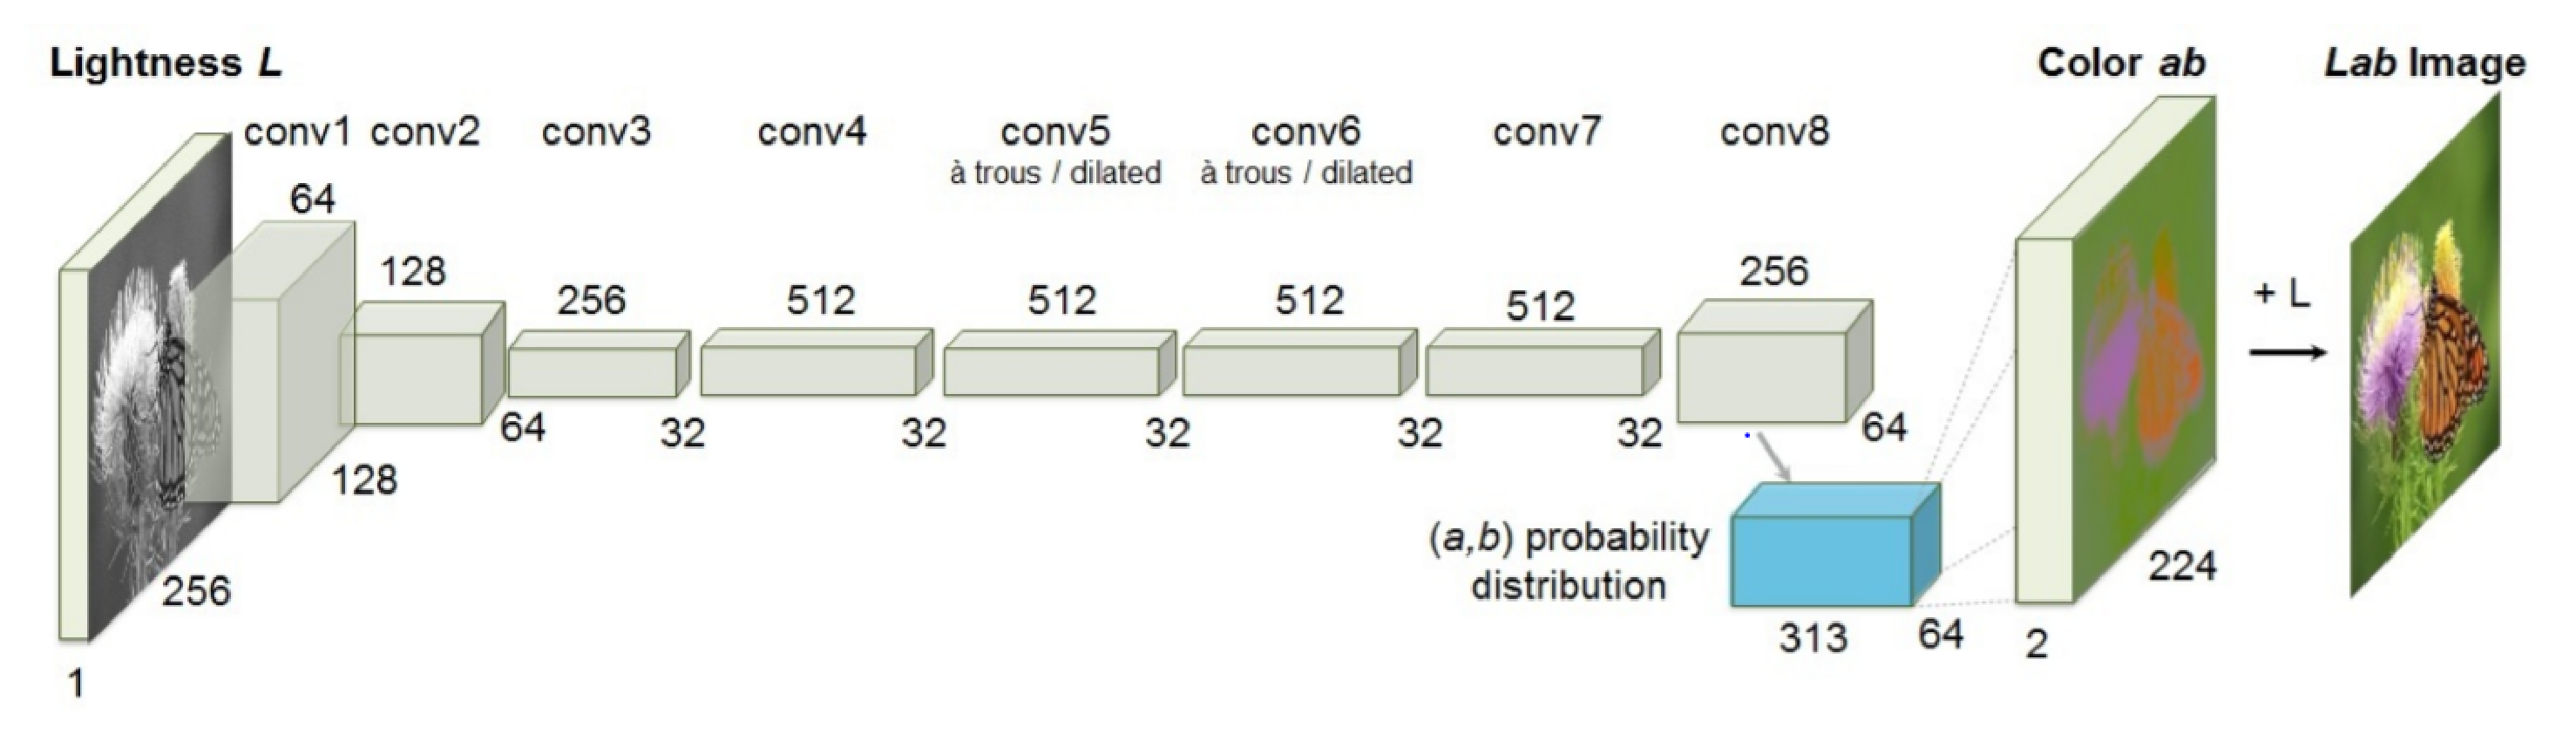
\includegraphics[width=0.7\paperwidth]{appendixF2}
  \caption*{图~2\quad 我们的网络结构。每个conv层代表2到3个重复conv和ReLU层的集合,跟着一个BatchNorm层。这个网络没有池化层。解决方案中所有的改变都来源于在卷积块之间的空间下采样和上采样。}
  \label{tab:badfigure2}
\end{figure}

\section{方法}
我们训练了一个CNN从灰度输入映射到量化颜色值输出的分布,使用图2所示的结构。结构细节在我们的项目网页的补充材料中给出了描述,且该模型是公开可用的。 接下来,我们专注于目标函数的设计,以及我们的用于从预测的颜色分布中推断点颜色的技术。

\subsection{目标函数}
给定输入的亮度通道$X \in \mathbb{R}^{H \times W \times 1}$,我们的目标是学习一个到两个相关联的彩色通道$Y \in \mathbb{R}^{H \times W \times 2}$的映射$\hat{Y} = \mathcal{F}(X)$,在这里$H, W$是图像的大小。(我们给预测结果加了一个$\hat{.}$标志而真实结果没有)我们在CIE Lab颜色空间上进行的这个任务。由于这个空间上的距离建模了视觉上的距离,在中使用的一个自然的目标函数,就是在预测结果的颜色和真实结果颜色之间的欧式距离$L_2(.,.)$:

\begin{equation}\tag*{(1)}
L_2(\hat{Y}, Y) = \frac{1}{2}\sum_{h,w}\|Y_{h,w} - \hat{Y}_{h,w}\|_{2}^{2}
\end{equation}

但是,这个损失在面对着色问题的固有模糊性和多模态时不够鲁棒。如果一个物体可以在取一系列的不同ab值,欧式距离损失的最优解就会是这些值的平均值。在颜色预测中,这种平均的效果倾向于灰色和不饱和的结果。另外,如果合理着色的集合是非凸的,那么平均结果可能会落在合理区域外,从而给出不合理的结果。

\begin{figure}[h]
  \centering
  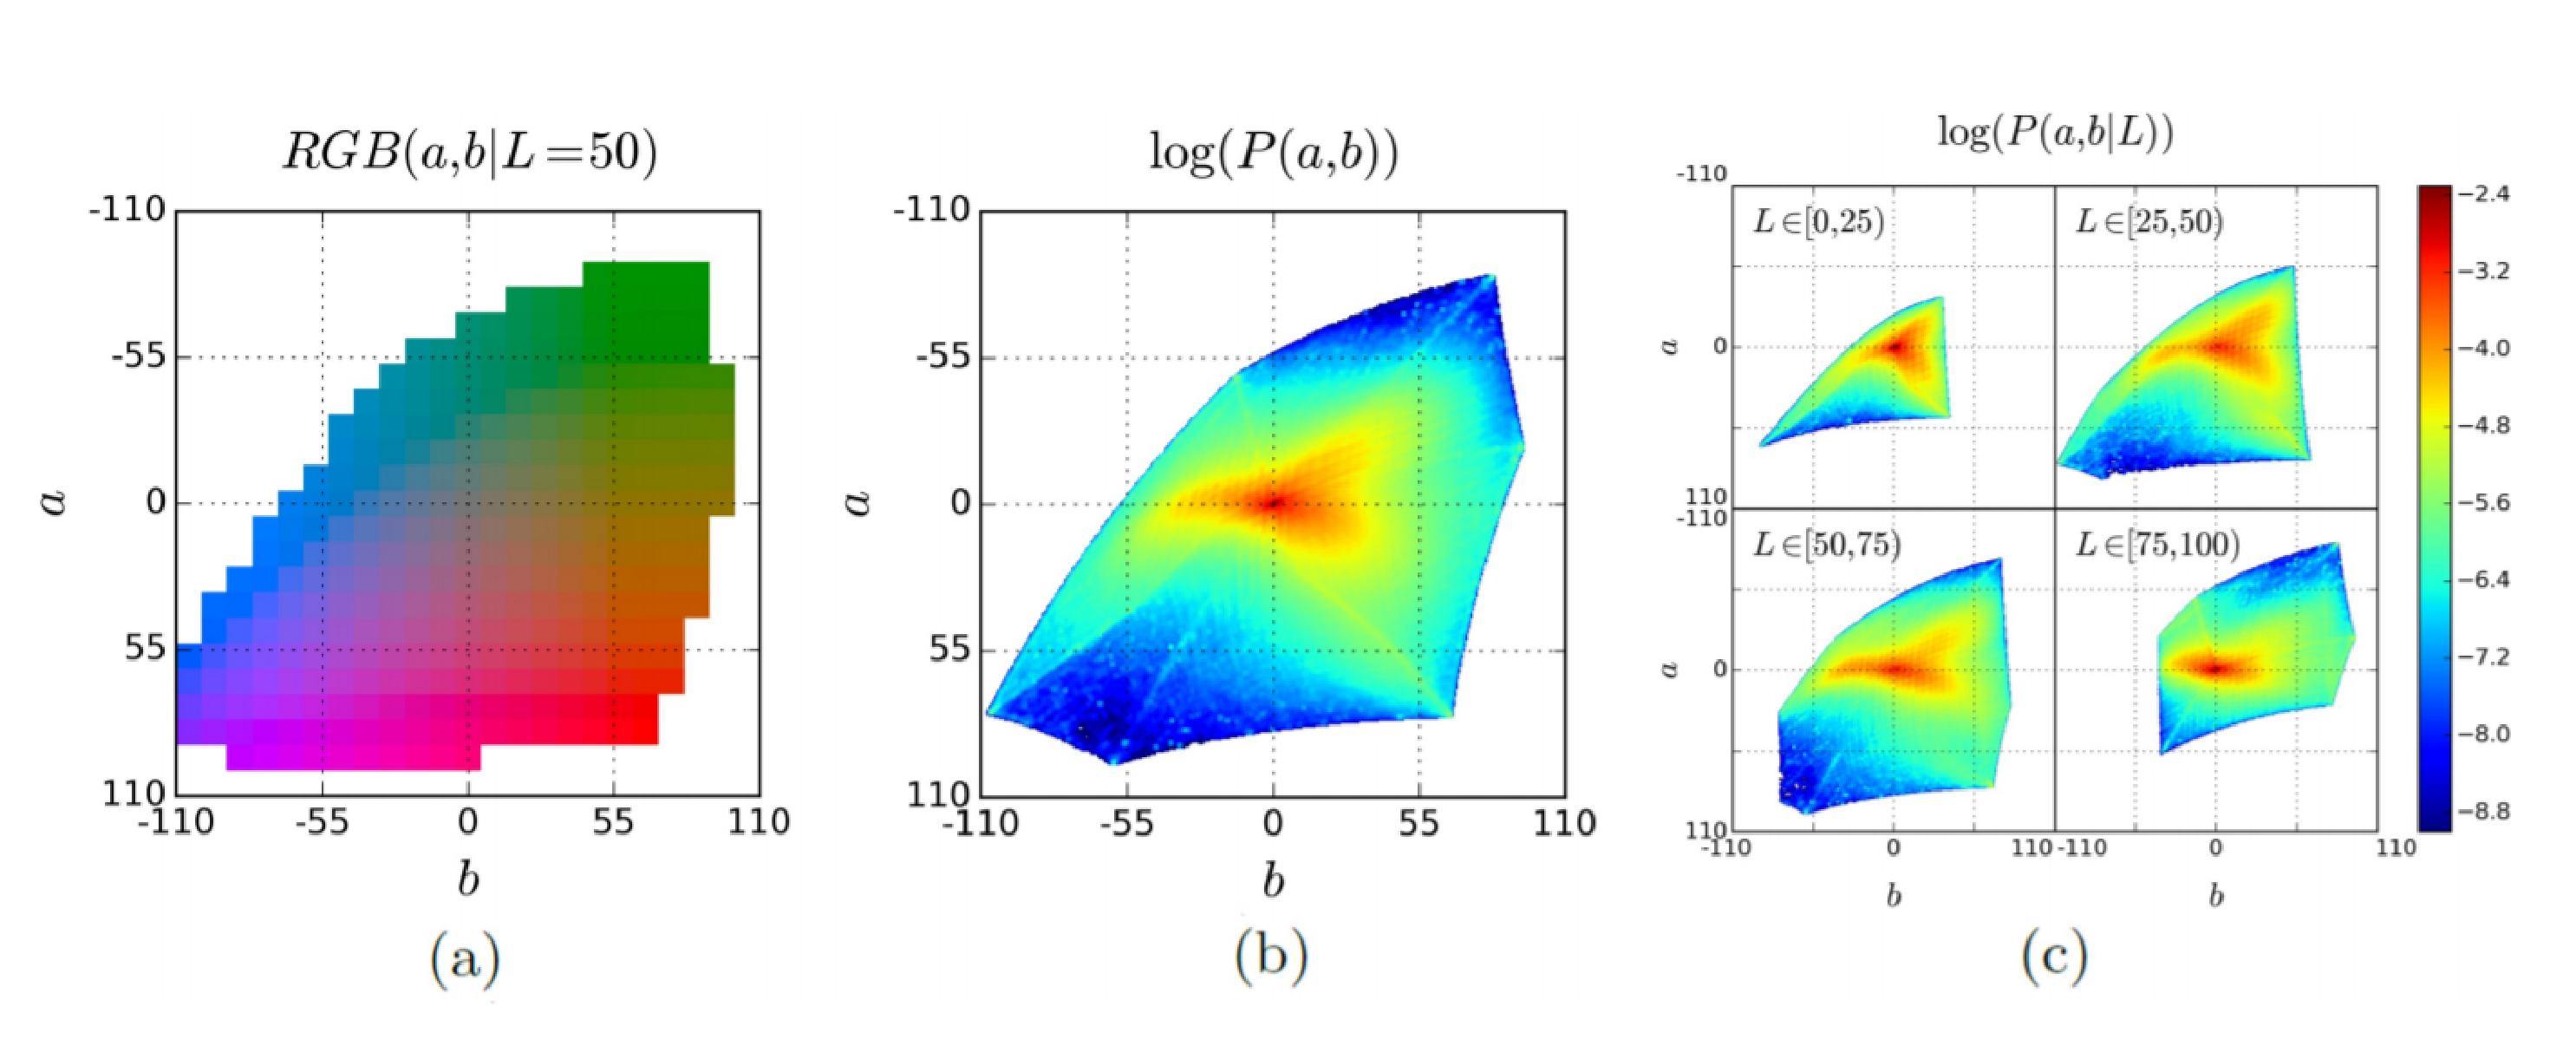
\includegraphics[width=0.7\paperwidth]{appendixF3}
  \caption*{图~3\quad (a)用大小为10的方格量化后的ab色彩空间。色域中总共包含313个ab色彩对。(b)ab颜色的经验分布,在log尺度下显示(c)在给定L值条件下的ab颜色经验分布,在log尺度下显示。}
  \label{tab:badfigure3}
\end{figure}

相反,我们把这个问题当成一个多模态的分类问题。我们将ab色彩空间量化为方格大小为10的桶并且保留了在色域的$Q = 313$个值,如图3(a)所示。对于给定的输入$Xs$,我们学习了一个到可能颜色$\hat{Z} \in ^{H \times W \times Q}$概率分布的映射$\hat{Z} = \mathcal{G}(X)$,在这里$Q$是量化后ab值的数量。

为了比较预测的结果$\hat{Z}$与真实结果,我们定义了一个将真实颜色$Y$转换到向量$Z$的函数$Z = \mathcal{H}^{-1}_{gt}(Y)$,使用的是软编码方案。我们然后使用了多模态的交叉熵损失$L_{cl}(.,.)$,定义为

\begin{equation}\tag*{(2)}
L_{cl}(\hat{Z}, Z) = -\sum_{h,w}v(Z_{h,w})\sum_{q}Z_{h,w,q} \log(\hat{Z}_{h,w,q})
\end{equation}

在这里$v(.)$是一个权重项,可以用来重新平衡稀有的颜色类别的损失,在下面的2.2节定义。最后我们用映射函数$\hat{Y}=\mathcal{H}(\hat{Z})$将概率分布$\hat{Z}$映射到颜色值$\hat{Y}$,这会在2.3节讨论。

\subsection{类别重新平衡}

由于背景的表现例如云朵,人行道,尘土和围墙,自然图片中的ab值的分布严重倾向于很低。图3(b)显示了在ab空间像素的经验分布,数据来源于ImageNet的130万张训练图片。观察到自然图片中的不饱和像素的数量比饱和像素的数量高出了几个数量级。如果不考虑到这一点,损失函数就会被不饱和ab值占据。我们通过在训练时基于像素颜色的稀有度重新加权了每个像素的损失来针对这个问题。这渐近地等同于典型的对训练空间重新采样的方法。每个像素被一个因素$w \in \mathbb{R}^Q$衡量,基于它最近的ab颜色桶。

\begin{equation}\tag*{(3)}
v(Z_{h,w}) = w_{q^*}, \text{where } q^* = \text{arg } \max\limits_{q} Z_{h,w,q}
\end{equation}

\begin{equation}\tag*{(4)}
w \propto ((1-\lambda)\tilde{p}+\frac{\lambda}{Q})^{-1},\text{ } \mathbb{E}[w] = \sum_{q}\tilde{p}_{q}w_q = 1
\end{equation}

为了获得平滑的经验颜色分布$\tilde{p} \in \Delta^Q$,我们从整个ImageNet训练集统计了经验的量化的ab空间的概率分布$p \in \Delta^Q$并且用一个高斯核$\text{G}_{\sigma}$将分布做了平滑处理。然后我们将这个分布用一个权值$\lambda \in $与一个标准分布混合,采取倒数并且归一化所以权重因子的期望是1。我们发现$\lambda = \frac{1}{2}$和$\sigma = 5$效果很好。在3.1节里我们将这个结果与没有做类别重新平衡的结果进行了对照。

\subsection{从类别概率到点估计}

最终,我们定义了$\mathcal{H}$,是从预测的分布$\hat{Z}$到ab颜色空间$\hat{Y}$的映射。一种选择是对于每个像素取其预测分布的最大值,正如图4中最右一列所示的两个例子。这提供了一种富有活力的着色结果但是有时会造成空间不连续的结果,例如大巴上的红色斑点。从另一方面,取预测分布的平均值会造成空间上连续但是不饱和的结果(图4中的最左列),呈现一种不自然的棕褐色调。这是不令人惊讶的,因为在做分类处理之后取平均值与使用欧式距离作为损失函数的回归架构有一样的问题。为了在以上两方面都取得最好的结果,我们通过调整参数T来内插softmax分布,并且取了结果的平均值。我们的灵感来源于模拟退火技术,因此称这个操作为取分布的退火平均值。

\begin{equation}\tag*{(5)}
\mathcal{H}(Z_{h,w}) = \mathbb{E}[f_T(Z_{h,w})], \text{ } f_T(z) = \frac{\exp(\log(z)/T)}{\Sigma_q\exp(\log(Z_q)/T)}
\end{equation}

设T=1使得这个分布没有改变,降低温度使得分布更突出一些极值点,而当$T \rightarrow 0$会得到分布的单热点编码。我们发现当温度T=0.38,如图4的中间一列所示,能捕捉到活力性同时也维持空间连续性。

我们最终的系统$\mathcal{F}$是CNN $\mathcal{G}$与退火平均值操作$\mathcal{H}$的结合体,前者对所有像素生成了概率分布,后者生成最终的着色结果这个系统不能完全端到端的训练,但是记住一点就是这个映射$\mathcal{H}$对每个像素独立操作,只包含一个参数,并且可以实现为CNN前向传递的一部分。

\begin{figure}[h]
  \centering
  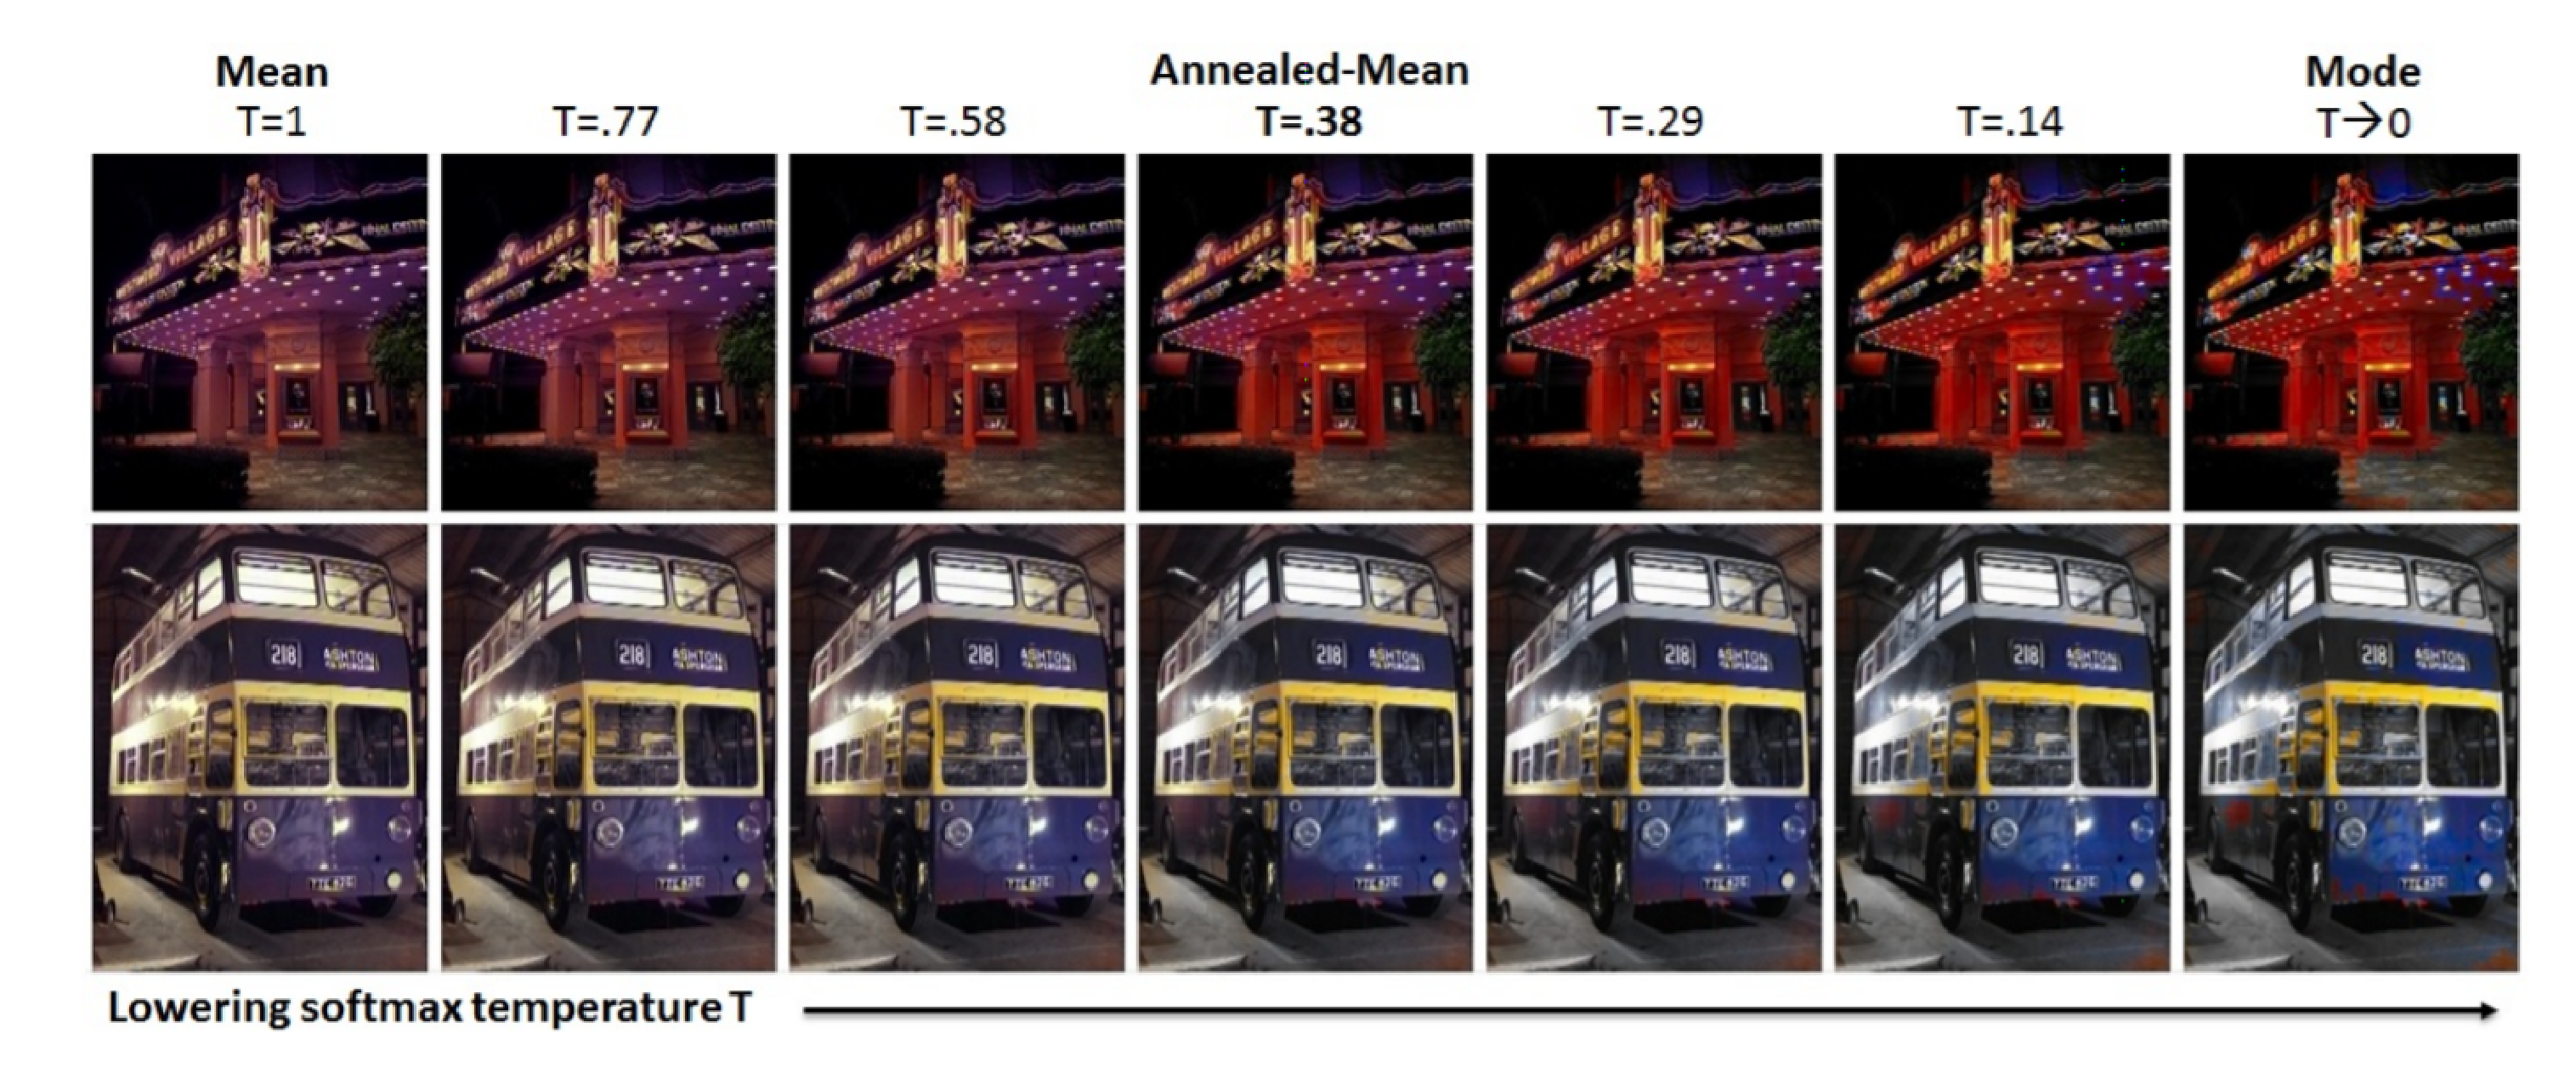
\includegraphics[width=0.7\paperwidth]{appendixF4}
  \caption*{图~4\quad 温度参数T对退火平均值输出的效果(公式5)最左边的图像是预测颜色的平均值,最右边的是取最可能的颜色值。在我们的系统中T=0.38}
  \label{tab:badfigure4}
\end{figure}

\section{实验}

在3.1节,我们在图像层面评估了我们的算法,评估了我们着色结果的视觉真实感,也使用了其他准确度评估方式。我们将自己完整的算法与几个变体以及最近和同时的工作做了对比。在3.2节,我们测试了着色作为一种自监督学习的方法。最后,在10.1节,我们展示了给真实老黑白照片着色的定性结果。

\begin{figure}[!htb]
  \centering
  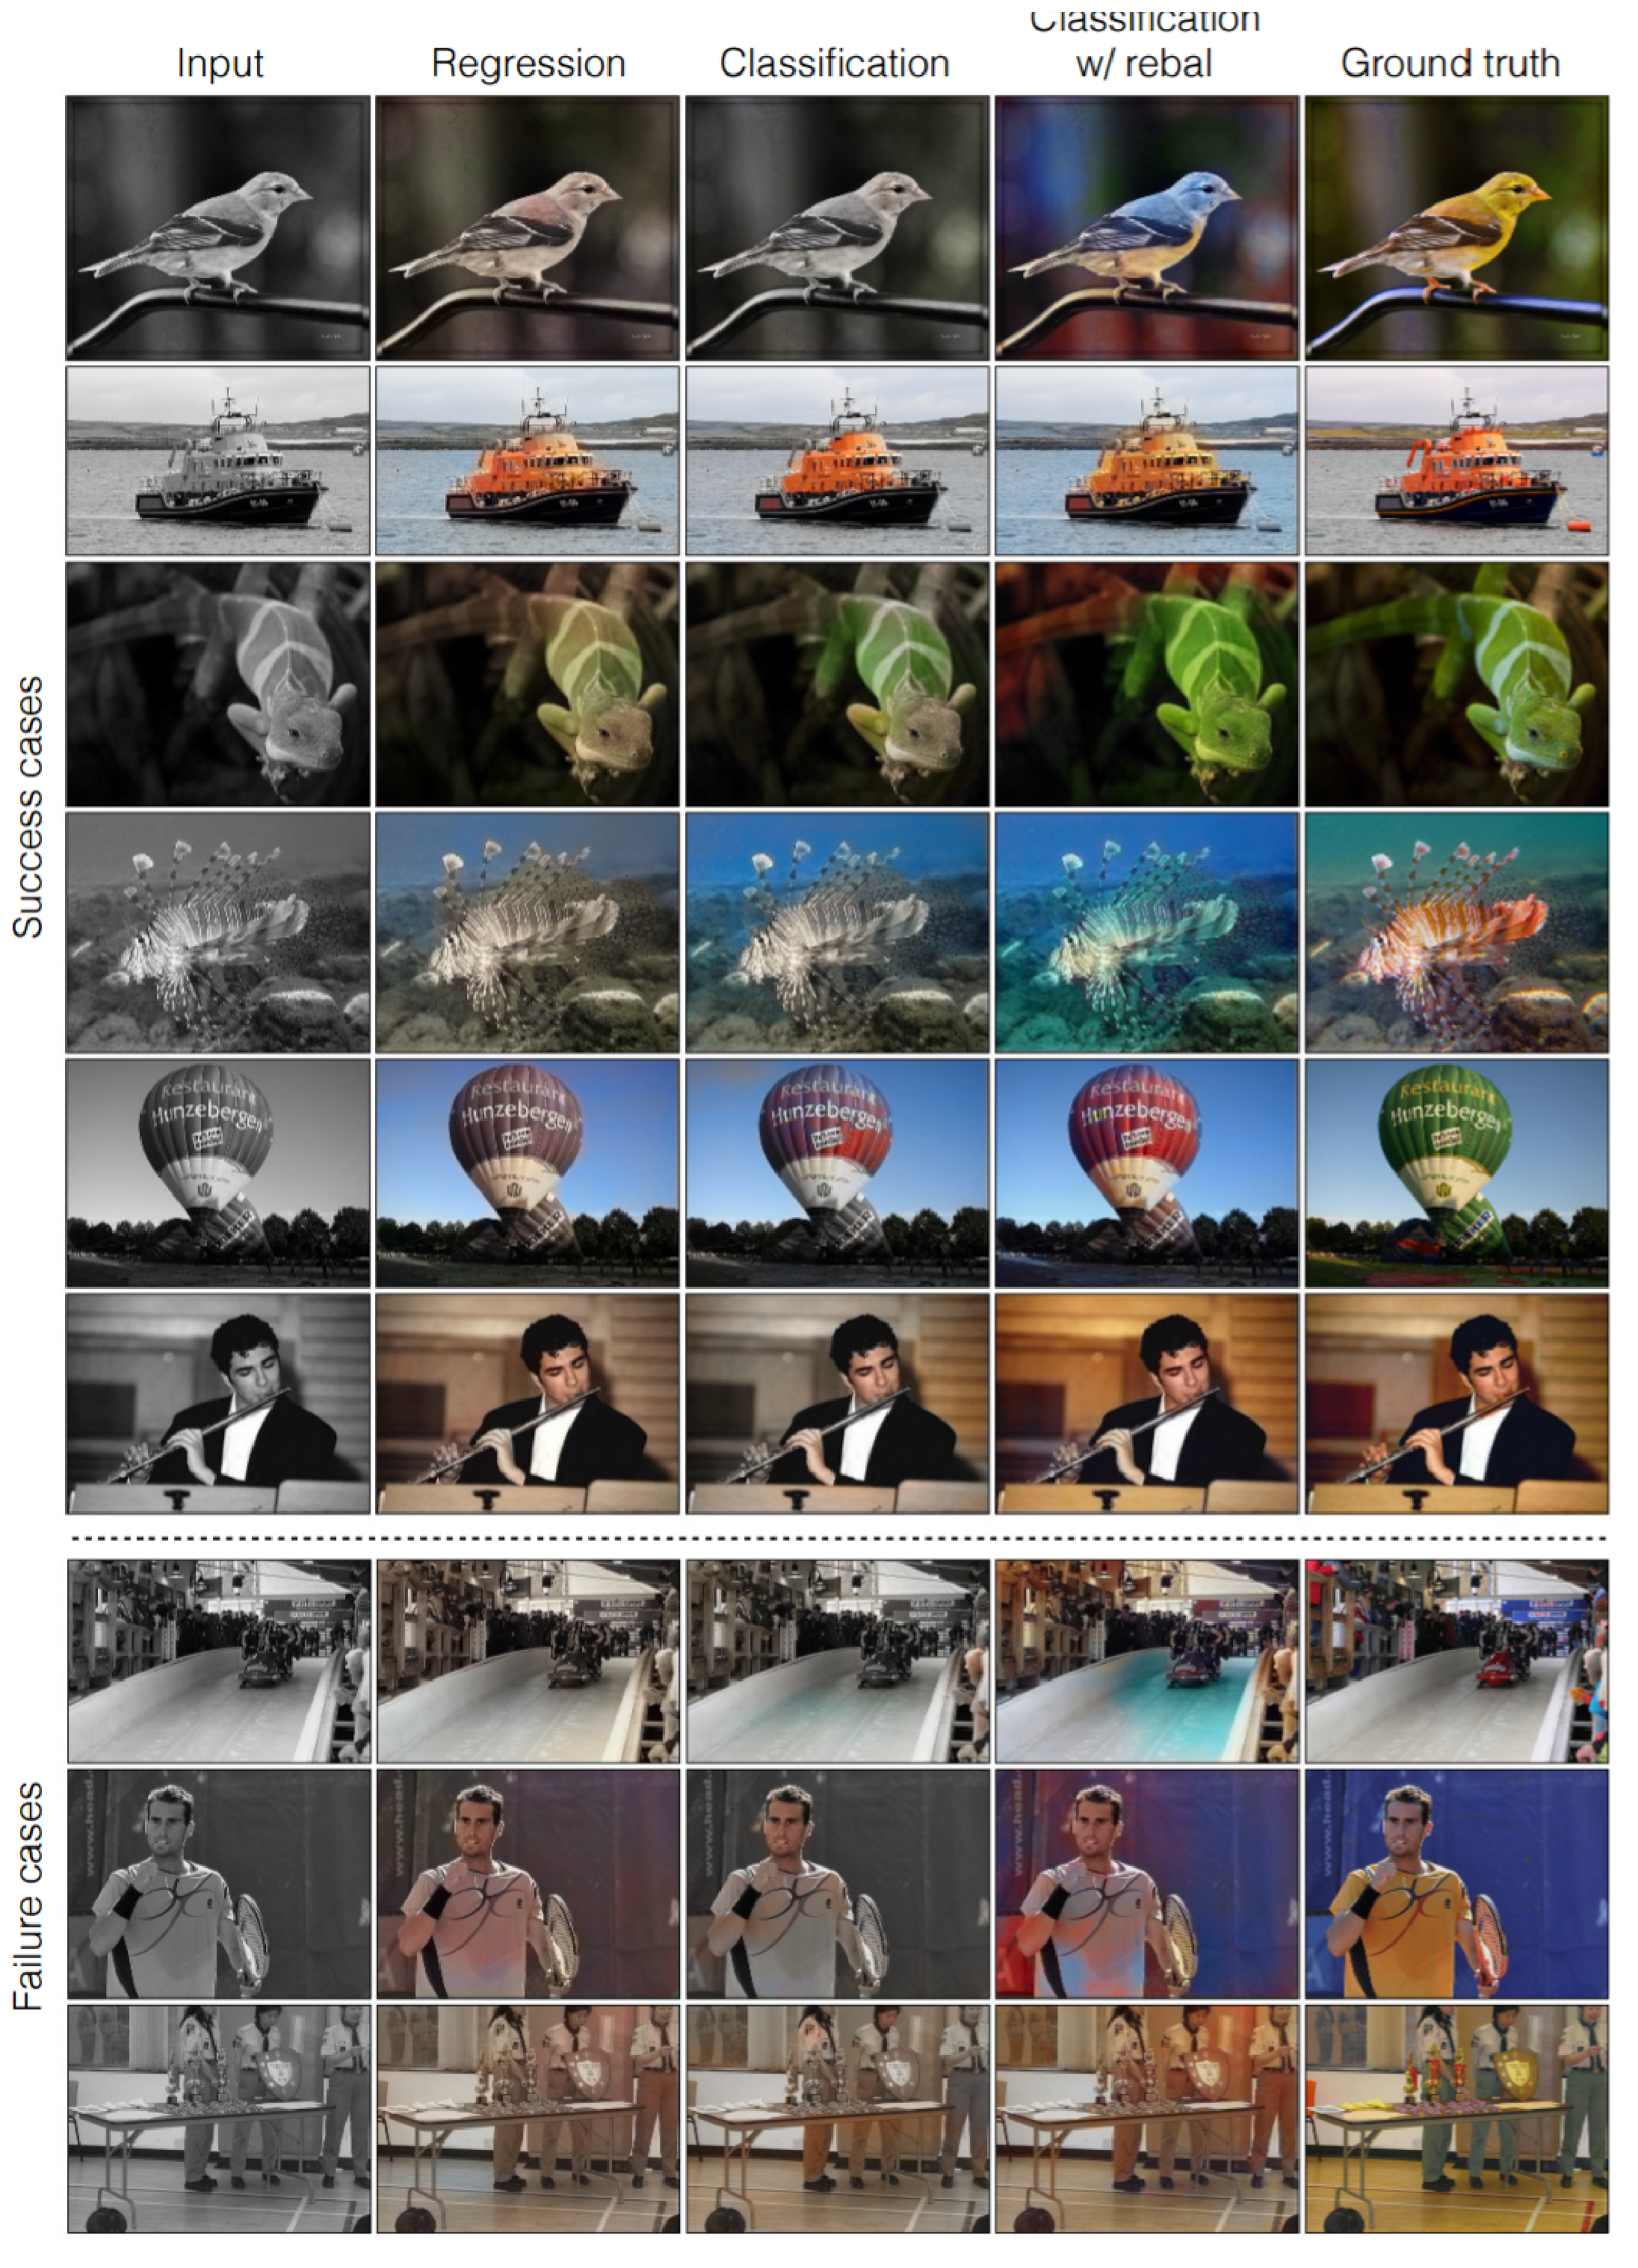
\includegraphics[width=0.6\paperwidth]{appendixF5}
  \caption*{图~5\quad 来自ImageNet测试集的结果。我们的分类损失和重新平衡比回归损或者没有重新平衡的分类损失制造了更准确和更有活力的结果。在点线上方是成功的着色,常见的失败案例在下方。其中包含不能抓取大范围连续性的失败,红色和蓝色之间的冲突,和室内场景的棕褐色调。访问\url{http://richzhang.github.io/colorization/}查看完整的结果。}
  \label{tab:badfigure5}
\end{figure}

\begin{figure}[h]
  \centering
  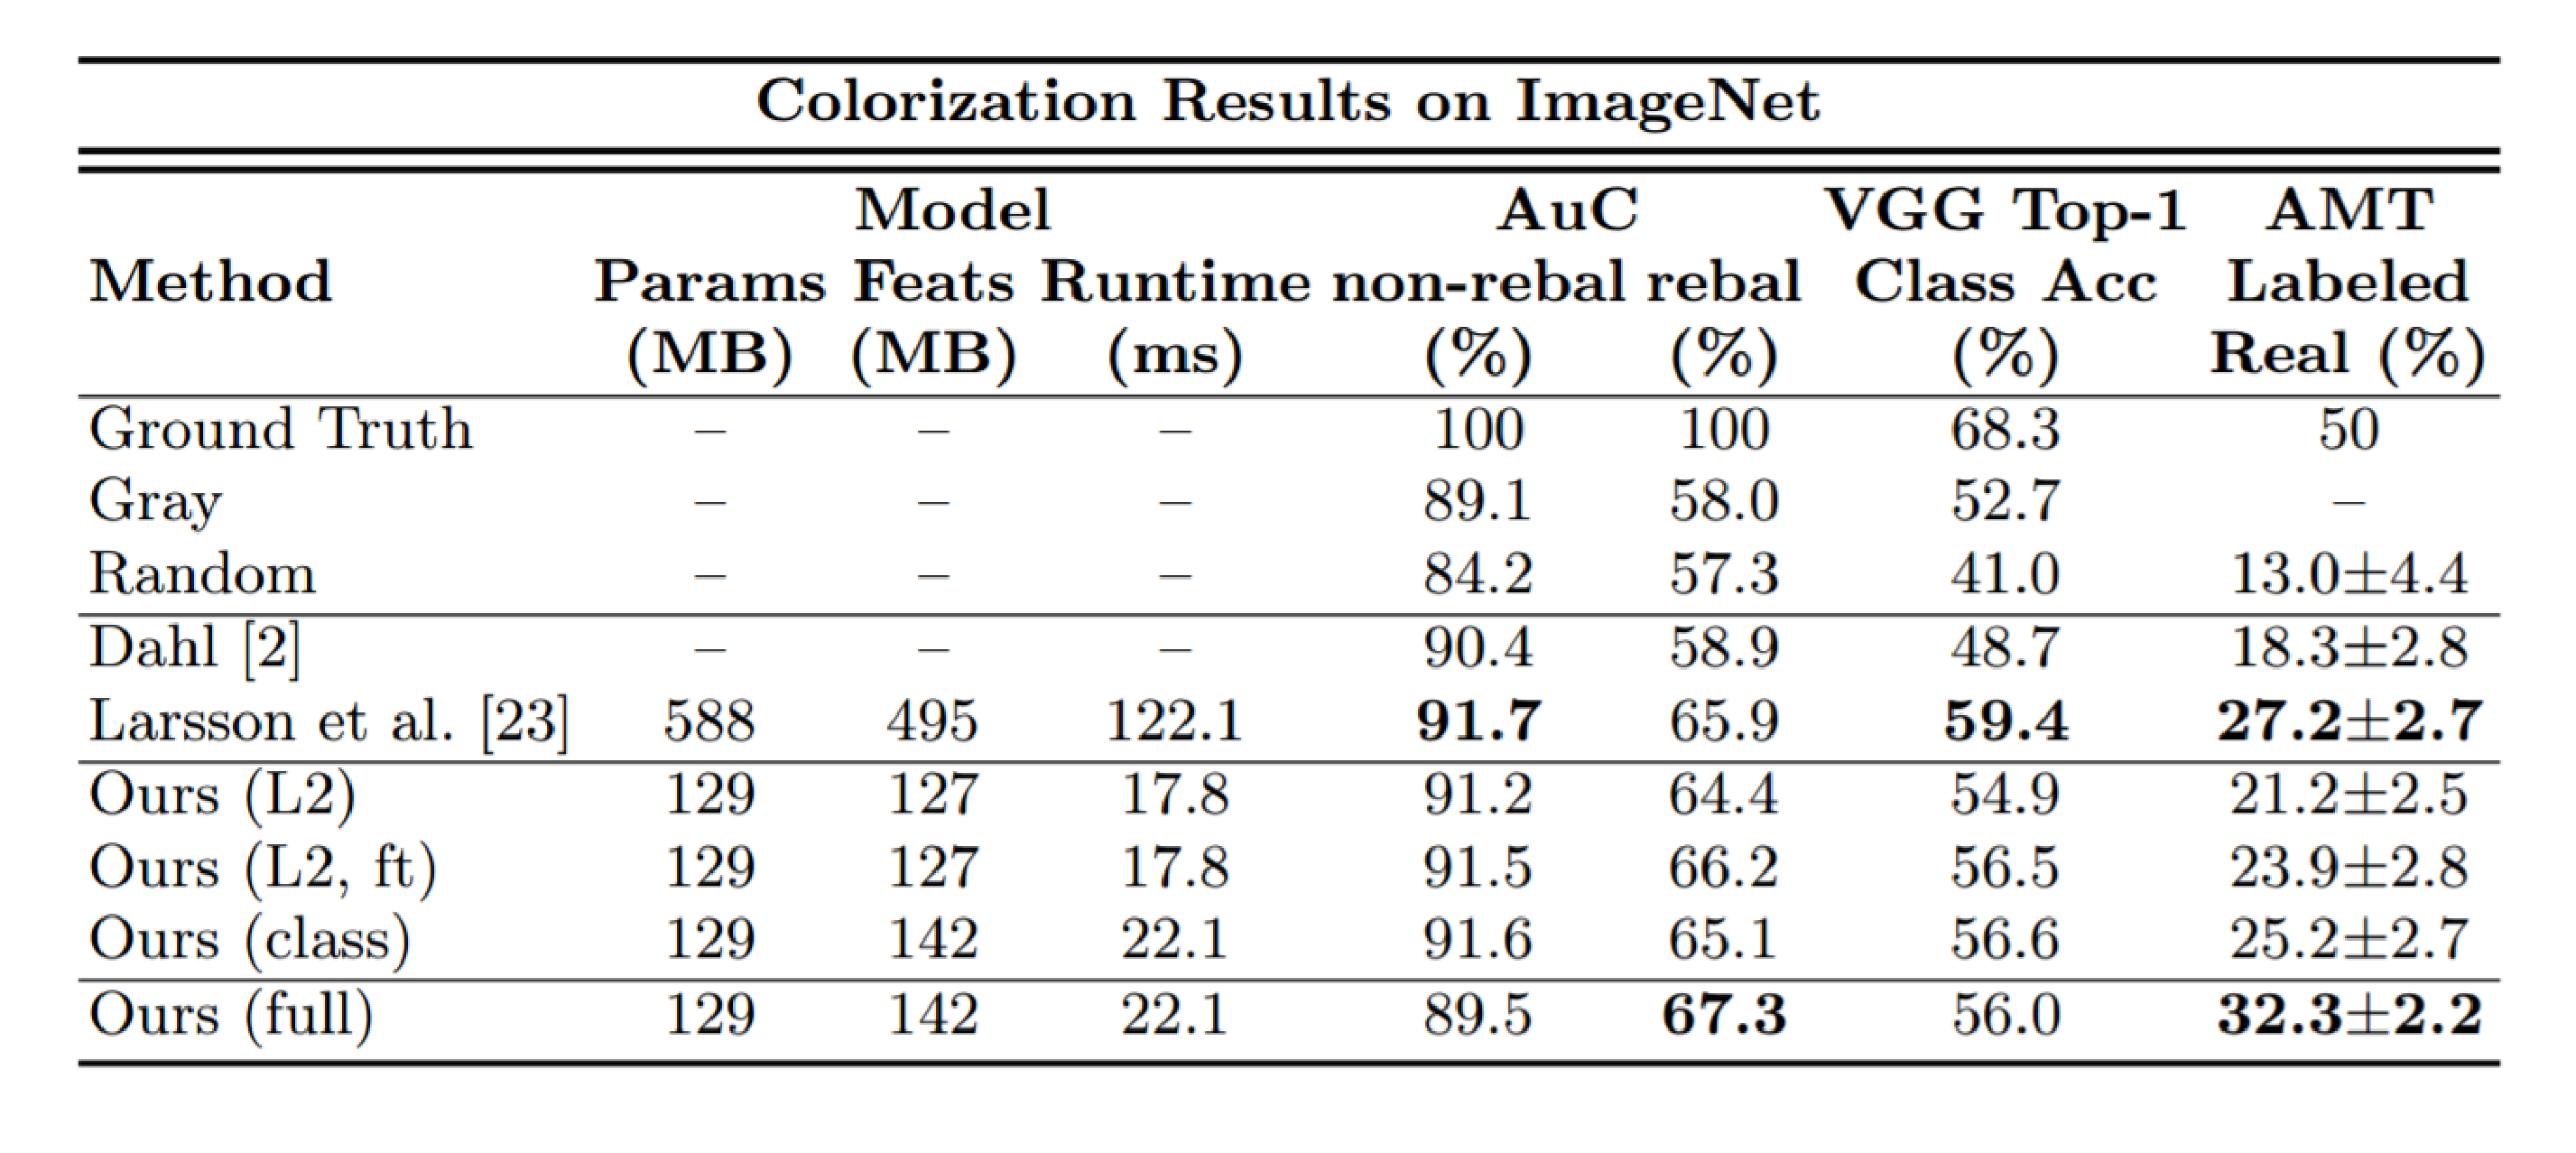
\includegraphics[width=0.7\paperwidth]{appendixT1}
  \caption*{表~1\quad 在ImageNet验证集上10k张图片的着色结果。AuC指的是曲线下方累积面积。第二列显示了类别平衡的结果。第三列是在着色后用VGG-16网络分类的准确率。第四列显示了我们在AMT上的真实vs虚假的测试(平均值和标准差都给出了)。注意使用两张真实照片期望上会得到50\%的准确率。所有标准都是数值越高越好。每一行表示不同的算法;请看每个算法的文字描述。参数,特征暂用内存以及运行时间在一块Titan X显卡上用Caffe测试}
  \label{tab:badfigure6}
\end{figure}

\subsection{评估着色质量}

我们在ImageNet训练集上的130万图片上训练了我们的网络,用ImageNet验证集上前一万张进行了验证,并且使用了独立于验证集的一万张图片做测试,跟中一样。我们将量化的结果展示在表1中,使用了三种评估方式。一种量化对比对于选择出的成功和失败的例子在图5中可以看到。要看随机图像选择的对比结果,请访问我们的项目网站。


为了特别地测试不同损失函数的效果,我们使用不同的损失训练了我们的CNN。我们也对比了之前与现在的方法,它们多使用了在ImageNet上训练的CNN,使用了简单的基准线。

1. {\heiti 我们的(完整)} 我们完整的方法,带有公式2中定义的分类损失,和2.2节中定义的类别重新平衡。这个网络用k均值初始化,使用ADAM求解器迭代了大约45万次。

2. {\heiti 我们的(分类)} 我们的网络,有分类损失函数,但没有类别重新平衡(公式4中$\lambda = 1$)。

3. {\heiti 我们的(L2)} 我们的网络,L2回归损失,如公式1描述,遵照一样的训练参数。

4. {\heiti 我们的(L2微调)} 我们的网络,L2回归损失,从我们的完整版本微调而来。

5. {\heiti Larsson等人} 一个CNN的方法,,在之前的处理中也出现过

6. {\heiti Dahl} 一个之前的方法,在VGG特征上使用拉普拉斯金字塔,使用L2回归损失训练

7. {\heiti Gray} 将每个像素上成灰色,即$(a,b)=0$

8. {\heiti 随机} 从训练集中随机选一张图片的颜色复制过来。

评估生成图像的质量是一个众所周知的难题,像一些简单的量化评测方法,比如RMS像素颜色差,经常不能抓取视觉真实感。为了解决这些独立评测方法的缺点,我们测试了三种测试不同感觉质量的方法,如表1所示。

1. {\heiti 感知真实(AMT): } 对于许多应用,比如图形学中的那些,着色的终极测试就是能否骗过人类观察者。为了测试这一点,我们在AMT(Amazon Mechanical Turk)上进行了一个真实vs虚假的两项强制选择的实验。实验中的参与者被展示了一系列的两张图片。每一对图片包括一张彩色照片和它的重新着色版本,用我们的算法或者其他基准线生成。参与者被要求点击那张他们认为是由计算机程序生成的虚假照片,并且在每一对测试之后,参与者有无限的时间回答。每一个单元测试包含10对练习(不包含到最后分析的结果中),以及40对测试。在练习阶段,参与者会获得他们的选择是否正确的反馈。40对测试时不会给出反馈。每个单元测试只测试一个算法,并且每个参与者被允许最多参与一个单元。总共有40个参与者评估了所有算法。为了确保所有的算法在相同环境下测试(例如,时间,人口统计等等),所有的单元都是同时分发给独立同分布的参与者。

\begin{figure}[h]
  \centering
  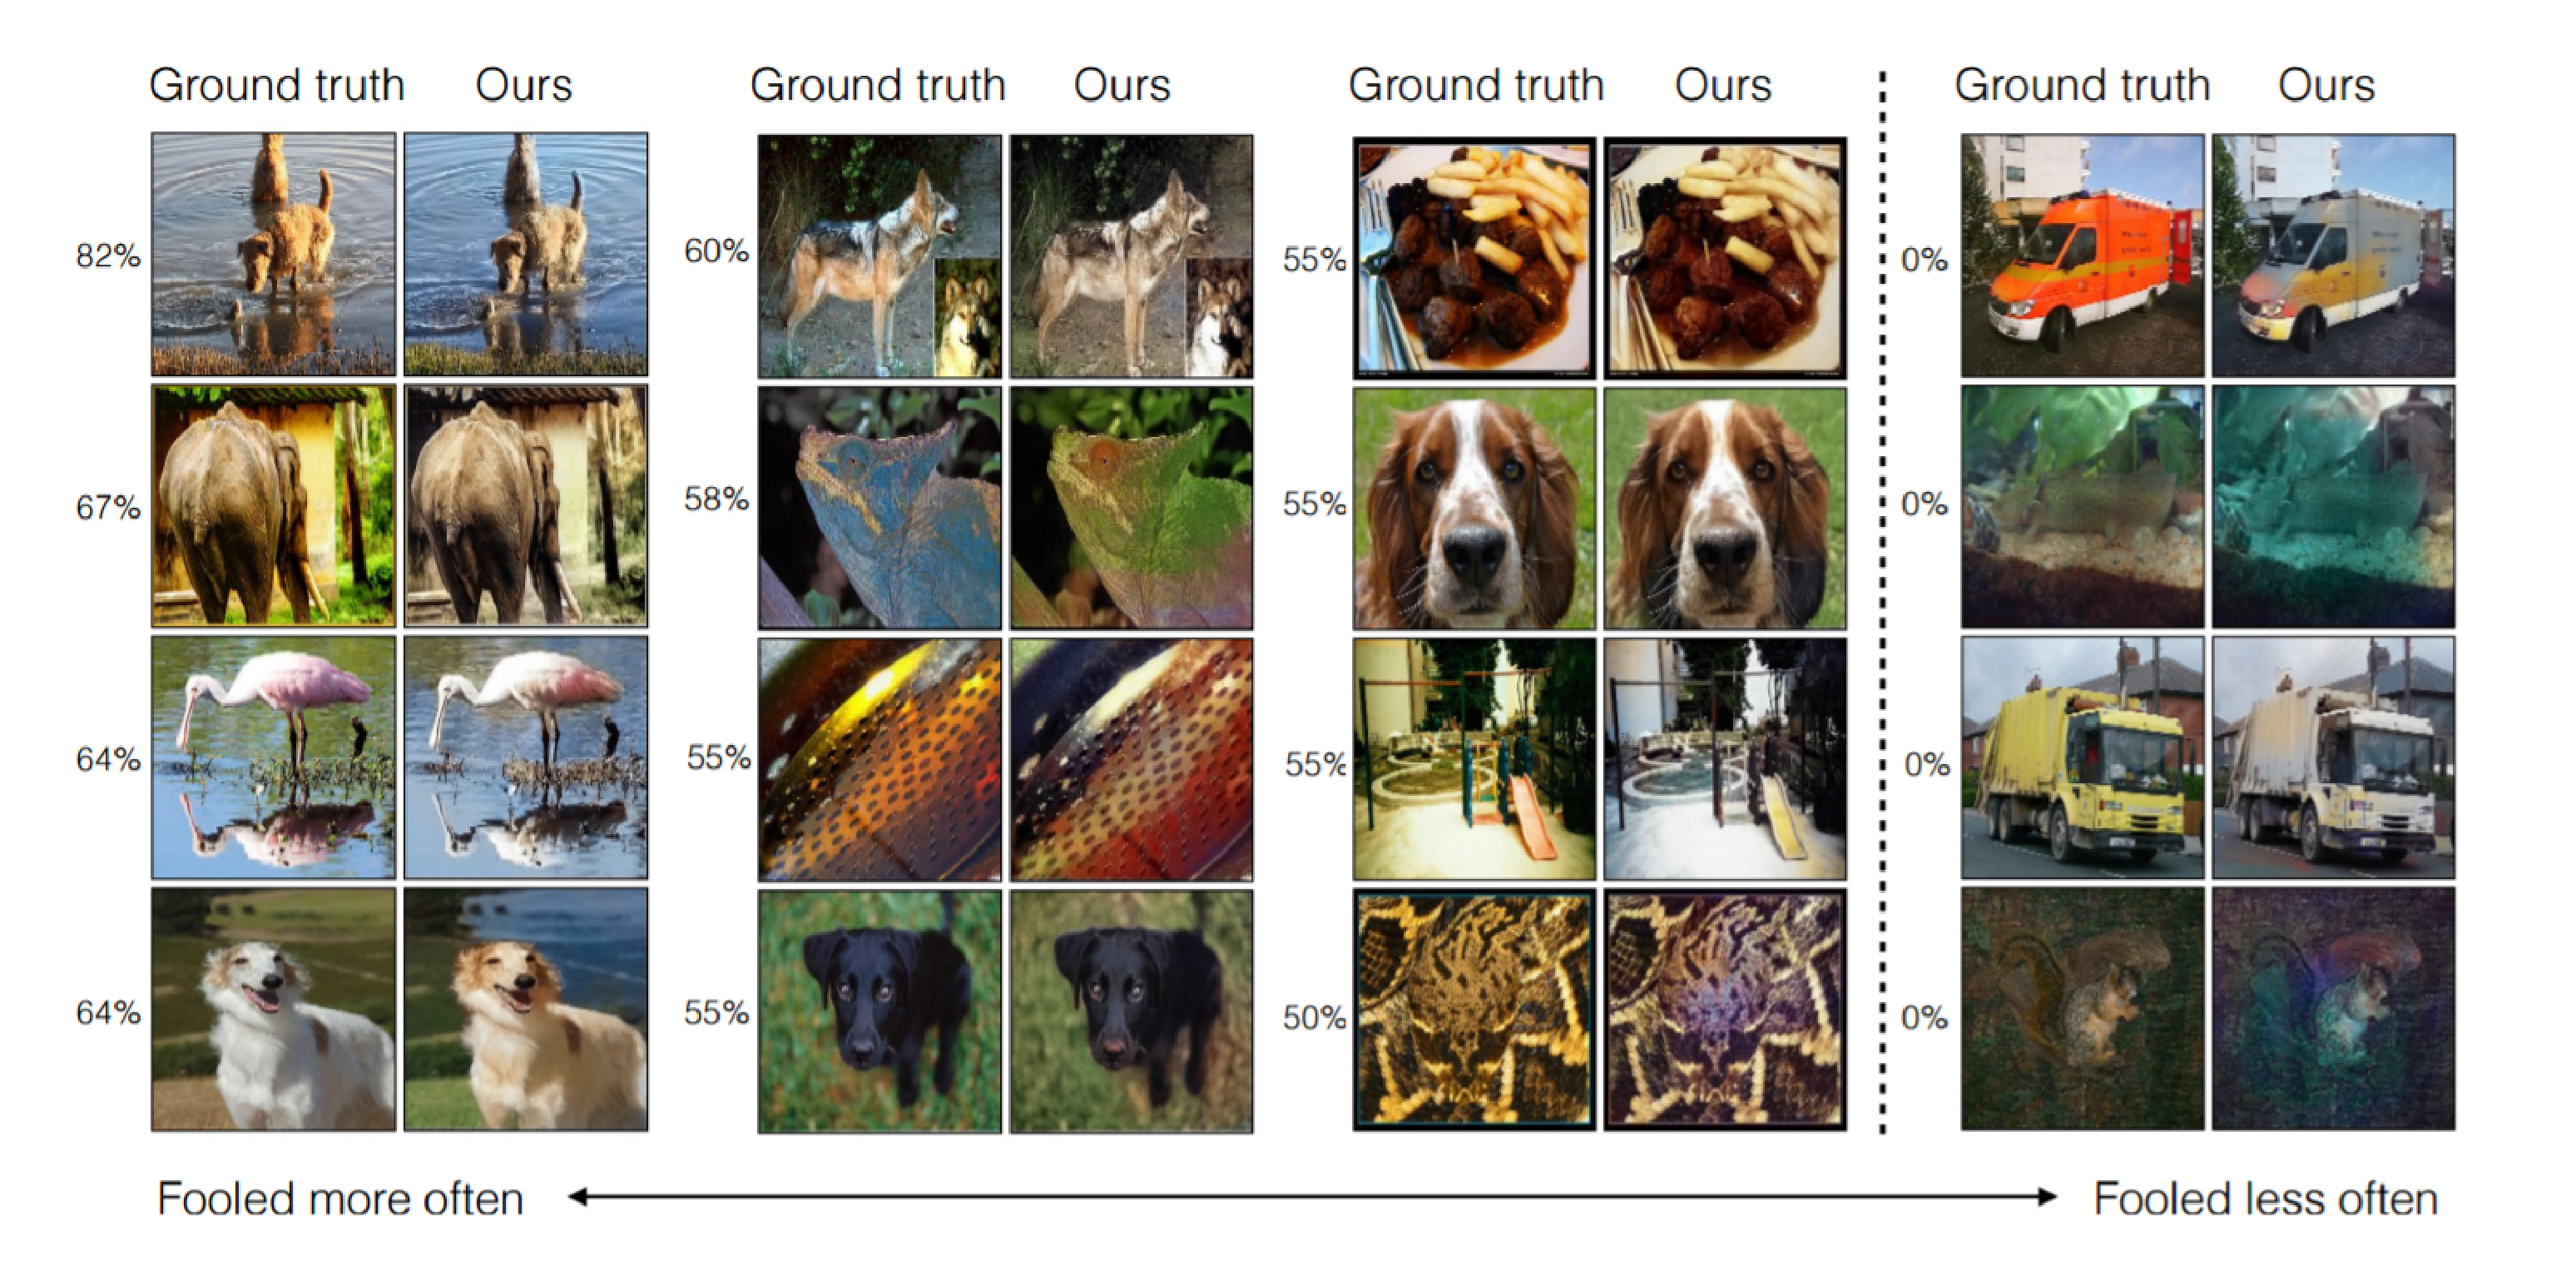
\includegraphics[width=0.7\paperwidth]{appendixF6}
  \caption*{图~6\quad 根据AMT测试者选择我们着色结果而不是真实图片的频率排序的结果。在所有点线左边的图像对,参与者在超过50\%的测试中相信我们的着色比真实图片更真实。在有些例子中,这可能是因为真实图片中糟糕的白平衡,而在被我们的算法修正后,显得更自然。点线的右边是参与者从来没被骗到的例子。}
  \label{tab:badfigure7}
\end{figure}

为了检验参与者在这个任务中是有可信度的,10\%的实验是针对真实照片与随机基准线的。参与者87\%的概率成功的认出了随机着色的图片,证明他们理解了这个任务并且在认真做。

图6给出了参与者在识别我们算法微妙错误的能力的更好的展示。最右一列显示的是那些参与者能100\%成功看出虚假照片的例子。每一对都被至少10个参与者打分。更仔细的观察可以看出在这些图片中,我们的着色算法给出了一些明显的人工痕迹,比如两辆卡车上的黄色斑点,损坏了照片的整体可信度。

但是,我们的完整算法在32\%的测试中欺骗了参与者,如表1所示。这个数字明显比参与比较的其他算法要高(在每个例子中p <0.05),除了Larsson等人的,与他们的差别不明显(p=0.10,所有的数据都由给出)。这些结果验证了使用分类损失和类别重新平衡都是有用的。

注意一点如果我们的算法完全生成了真实照片的结果,在两张一样图片之间的强制选择,会导致参与者被骗的期望概率是50\%。有意思的是,我们有一些例子中参与者有超过50\%的概率被欺骗,表示我们的结果比真实照片更真实。有一些例子在图6的前3列给出。在许多例子中,真实照片的白平衡不好或者有一些不真实的色彩,而我们的系统给出了更实际的表现。

2. {\heiti 语义可解释性(VGG分类): } 我们的方法生成的着色结果对于现有的物体识别器是否足够真实呢?我们通过将我们生成的虚假着色图片输入一个被用于ImageNet分类的VGG网络测试了这一点。如果这个分类器表现好,说明我们的着色对物体类别提供了足够准确的信息。使用一个现成的分类器去评测合成数据的真实性在中已经提出来过。

结果显示在表1的右起第二列中。在去除输入图片的颜色后,分类准确率从68.3\%降到了52.7\%。而在用我们的算法重新着色后,准确率提升到了56.0\%(我们方法的其他变种到达了一些稍高的结果)。Larsson等人的方法在这个测试中达到了更好的结果,59.4\%的准确率。作为参考,一个在灰度输入上微调过的VGG分类网络可以达到63.5\%的结果。

除了作为一个感知评估标准,这个分析指出了我们算法的一种实际用处:不需要额外的训练或者微调,我们就能改善灰度图片分类的结果,只要用我们的算法着色然后输入到一个现成的分类器中。

3. {\heiti 原始准确率(AuC): } 作为一个低端的测试,我们计算了生成图片像素与真实图片像素ab颜色L2距离在一定阈值内的百分比。然后我们设置阈值从0到150以生成一个累积质量函数,如所说,对曲线(AuC)下的区域求和,并且归一化。注意这个AuC方法测试的是原始预测的准确率,而我们的方法目标是合理性。

我们的网络,分类训练而没有类别重新平衡时,要远好于L2变种(当从头开始训练)。当L2网络从颜色分类网络微调而来,它可以达到分类网络的表现。这表明L2可以达到准确的着色,但是从头开始训练会很难达到最优。Larsson等人的方法达到了稍微好一点的准确率。注意到这个评估方法充满了不饱和的像素,由于ab颜色在自然图像中的分布(图3(b))。结果就是,即使将每个像素预测为灰色也能得到很好的评价,而我们的完整算法也得到类似的分数。

另一方面,图像中的感兴趣的区域倾向于有一个更高饱和度的ab值分布。如此,我们计算了一个类别平衡版本的AuC,通过重新加权像素的颜色概率(公式4,设$\lambda = 0$)。在这样的评估下,我们的完整算法远优于所有变种和其他比较的算法,显示对训练物体做类别重新平衡达到了预计的效果。

\begin{figure}[h]
  \centering
  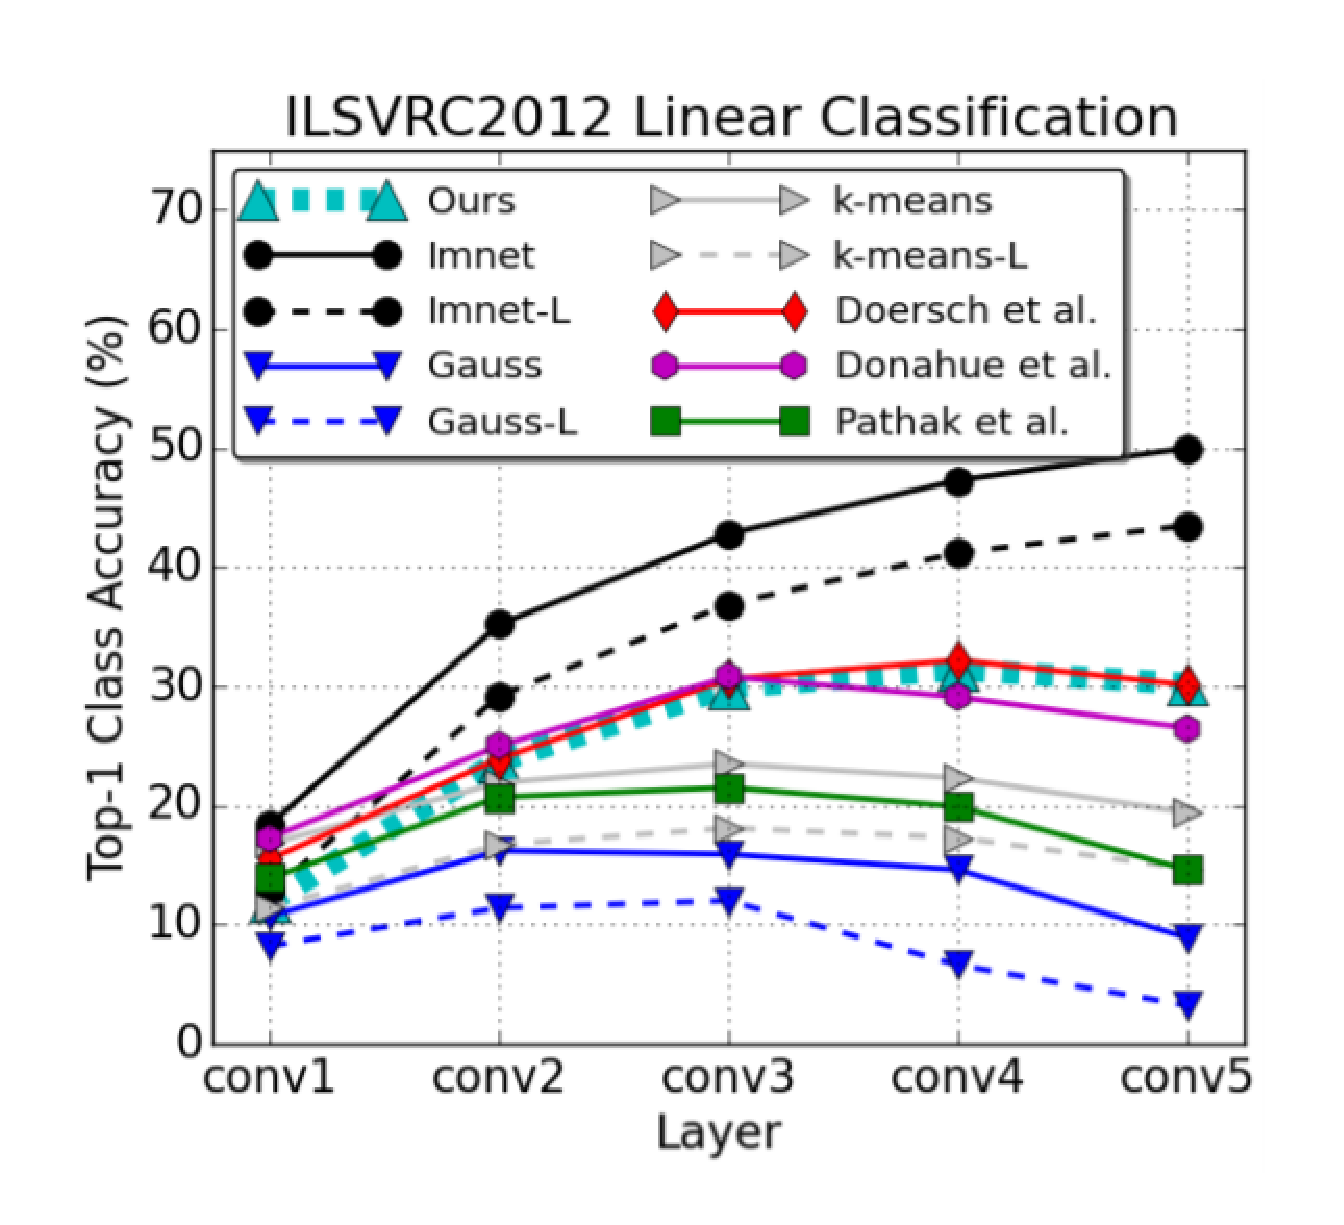
\includegraphics[width=0.7\paperwidth]{appendixF7}
  \caption*{图~7\quad {\heiti ImageNet上的任务综述} 我们固定了预训练的网络并且为ImageNet分类学习了线性分类器。特征被平均池化和相等的核和步幅大小,直到特征维度小于10k。ImageNet,k均值,以及高斯初始化在灰度输入上运行,用点线表示。彩色输入的结果用连续线给出。之前的和现在的工作自监督方法都展示了。}
  \label{tab:badfigure8}
\end{figure}

\begin{figure}[h]
  \centering
  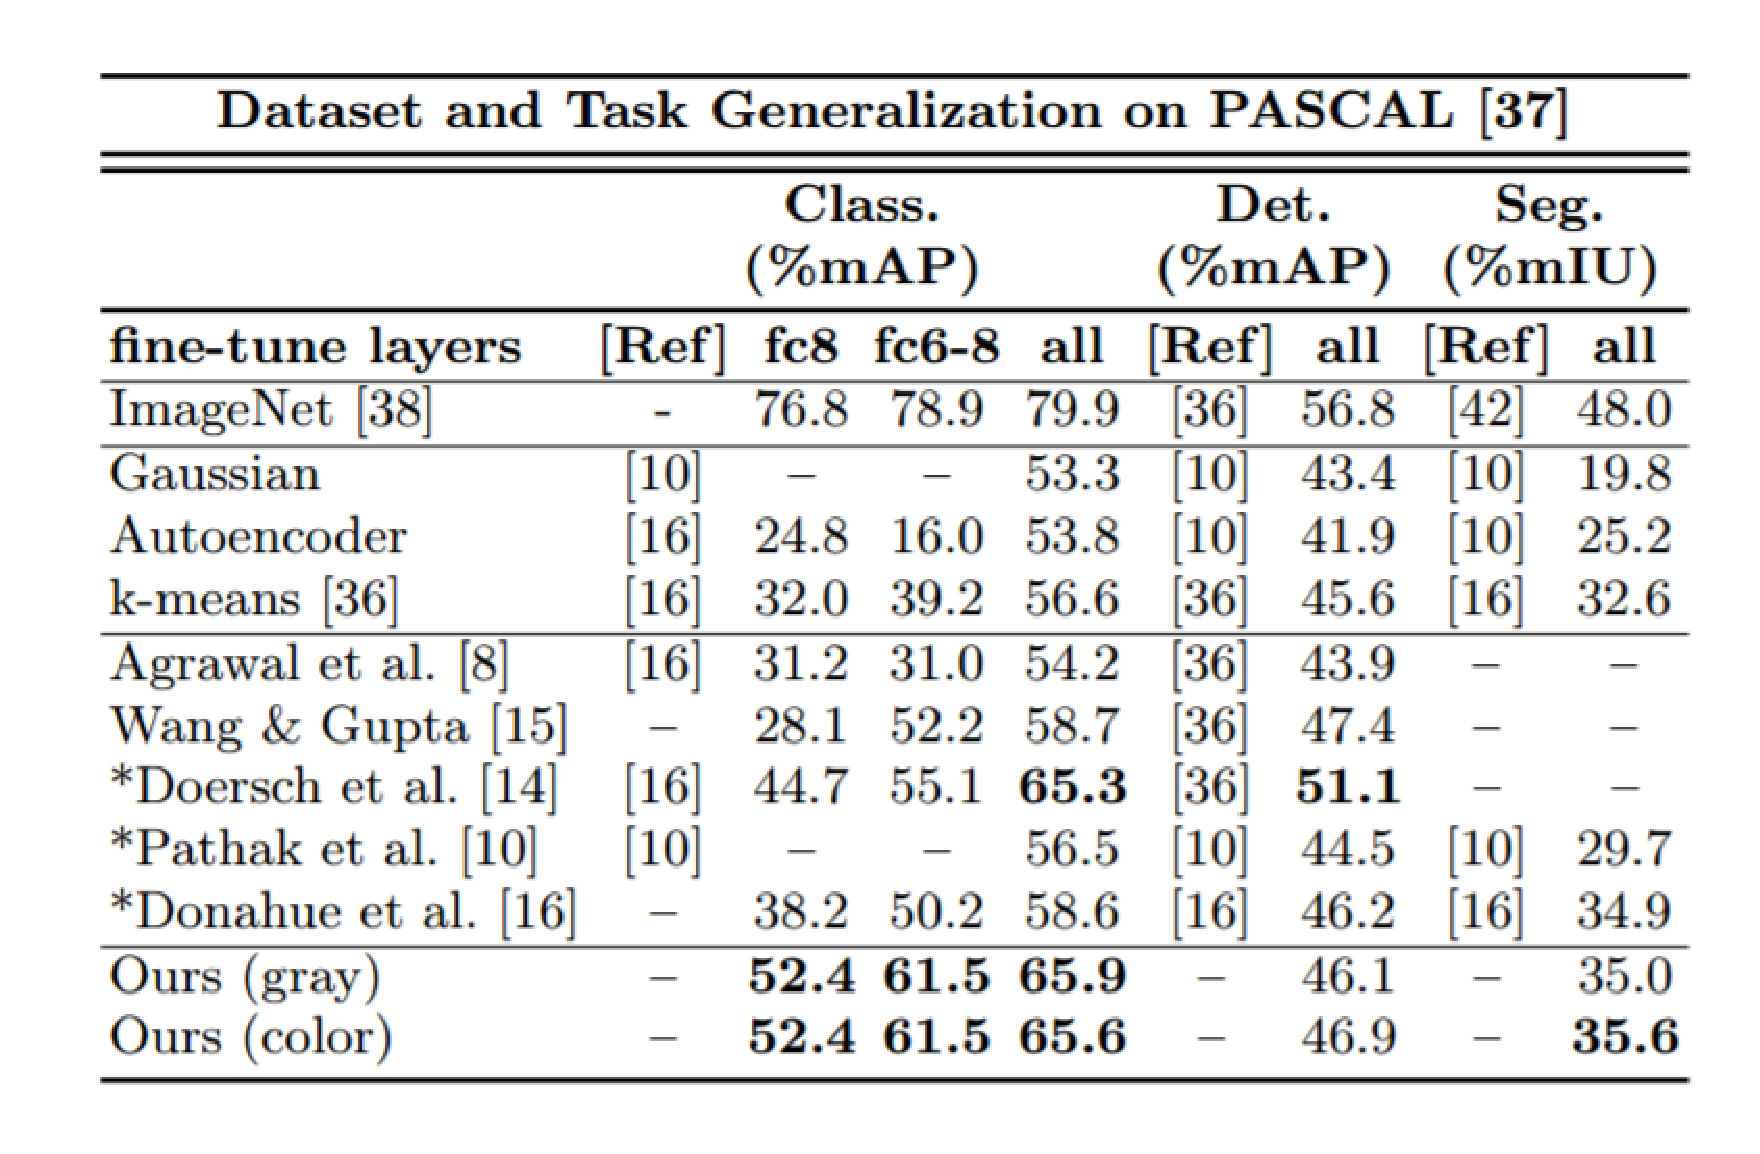
\includegraphics[width=0.7\paperwidth]{appendixT2}
  \caption*{表~2\quad {\heiti PASCAL 上的任务和数据集} PASCAL VOC 2007上的分类和检测任务以及PASCAL VOC 2012上的分割任务,为每个任务使用了标准平均准确率(mAP)和集合平均交集。我们对灰度输入和彩色输入微调了网络。带*的方法只预训练了AlexNet层的子网络。余下的层用初始化。}
  \label{tab:badfigure9}
\end{figure}

\subsection{交叉通道编码作为自监督特征学习}

除了在着色任务上做出了贡献,我们评估了着色如何作为表示学习的前文工作。我们的模型类似于自动编码,除了输入输出是不同的图像通道,于是有术语交叉通道编码。

为了评估通过这种交叉通道编码学习的特征表示,我们在我们的网络上跑了两组测试。首先,我们测试了这个特征的任务泛化能力通过固定学习表示和在已经见过的数据上(图7)训练线性分类器。第二,我们在PASCAL数据集上微调了网络,以适用于分类,检测和分割的任务。在这里,除了在已有的任务测试,这组实验还测试了学习表示的数据泛化能力。为了与之前的特征学习算法公平比较,我们在着色任务上重新训练了一个AlexNet网络,使用我们完整的方法迭代了45万次。我们发现结果在物体分类和分割上相比之前的方法达到了更好的表现(表2)。

{\heiti ImageNet分类 } 这个网络是在ImageNet数据集上预训练着色的,没有语义标签的信息。我们测试了学习的特征能多大程度代表物体层面的语义。为了达到这个效果,我们固定了网络参数,提供语义标签,并且在每个卷积层训练线性分类器。结果如图7所示。

在ImageNet分类上直接训练的AlexNet达到了最好的结果,并且为这个测试设立了一个最高标准。随机初始化,用高斯权重或者在中实现的k均值方案,在中间层达到峰值。因为我们的表示是在灰度图片上学习的,在网络的输入上有障碍。为了量化这种信息丢失的影响,我们在灰度图分类上微调了AlexNet,并且采用了随机初始化。有趣的是,对所有三种方法,在彩色和灰度输入之间有6\%的性能差别,这一点在整个网络大致恒定。

我们比较了自己的模型和其他最近在ImageNet上预训练的自监督方法。	首先,我们的conv1表示相比其他竞争方法在线性分类性能上表现更差,但是使用灰度输入时是性能相近的。但是,这个性能差在conv2时立即消失了,我们的网络与其他方法整个网络相比达到了同等的性能。这表明尽管有输入障碍,解决着色任务鼓励在训练数据分布中线性的分离语义类别。

{\heiti PASCAL 分类,检测和分割 } 我们在通用的自监督基准PASCAL分类,检测和分割上测试了我们的模型。结果如表2所示,我们的网络在所有三个任务中都有很强的表现,并且在分类和分割中有最先进的表现。我们使用了的方法,其中调整层的尺度为了让他们能在同样的速率学习。我们在两种模式测试了自己的模型:(1)通过忽略颜色信息保持灰度输入(2)将conv1改成接受3通道Lab输入,初始ab通道的权值为0。

我们首先在PASCAL VOC 2007上测试了网络分类,遵照中的规定。网络通过固定一部分,微调剩下的来训练。注意当conv1固定时,这个网络只能有效的解释灰度图像。在所有的三个分类测试中,我们达到了最好的准确率。

我们同样在PASCAL VOC 2007上测试了检测任务,用快速R-CNN,遵照中的流程。Doersch等人达到了51.1\%,而我们使用灰度和彩色输入分别达到了46.9\%和47.9\%。我们的方法远高于强k均值基准线的45.6\%,但是所有的自监督方法依然远落后与在ImageNet上用语义监督预训练的56.8\%的结果。

最后,我们在PASCAL VOC 2012上测试了语义分割,使用的FCN架构,遵照中的规定。我们的着色任务与语义分割任务有相似之处,因为两者都是逐像素的分类问题。我们的灰度微调网络达到了35\%,与Donahue等人的结果相近,添加颜色信息后性能提升到了35.6\%,高于其他测试的算法。

\begin{figure}[h]
  \centering
  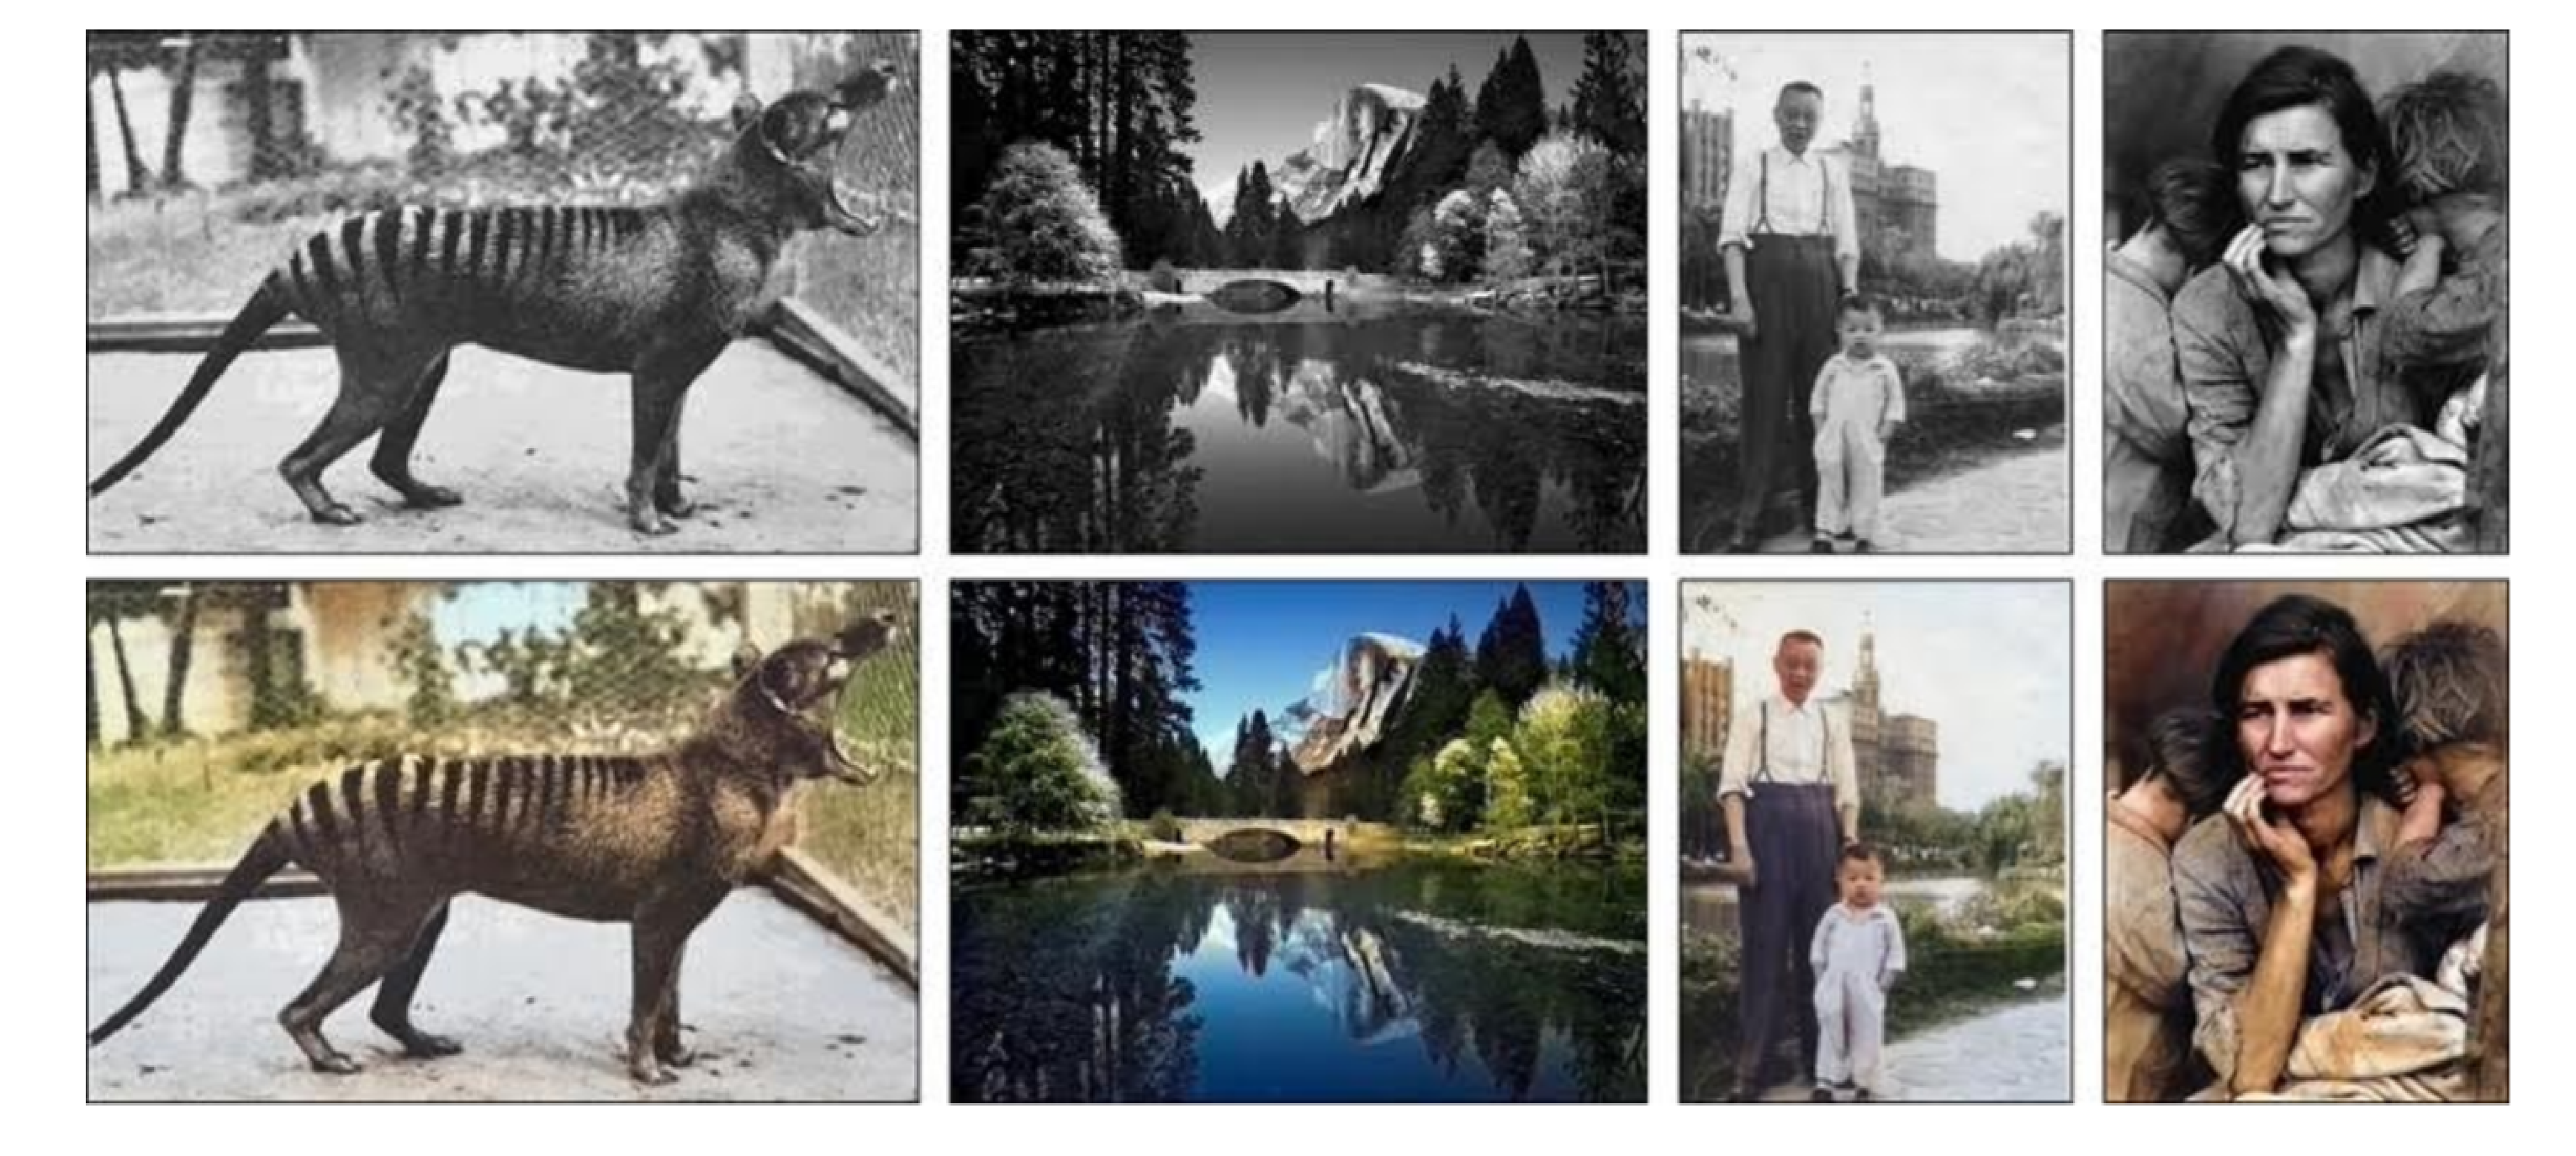
\includegraphics[width=0.7\paperwidth]{appendixF8}
  \caption*{图~8\quad 将我们的算法应用于传统黑白照片。从左到右:David Fleay拍摄的Thylacine,1936;Ansel Adams拍摄的优胜美地;业余爱好者的家庭照,1956;Dorothea Lange的移民母亲,1936}
  \label{tab:badfigure10}
\end{figure}

\subsection{传统黑白老照片}

由于我们的模型是用假的灰度照片训练,因为这些照片是用彩色照片去掉ab通道得到,所以我们也在传统黑白老照片上测试了我们的方法。如图8所示(更多结果可以在我们的项目网页上看到)。可以看出我们的模型依然能够产生良好的着色,尽管照片的低级统计数据与用来训练的现代照片有很大差别。

\section{结论}

虽然图像着色是计算机图形学中的精品任务,它也是计算机视觉中一个困难的像素预测问题。在这里我们展示了使用一个深层CNN与一个精心选择的目标函数能使着色达到与真实照片更近更难区分的结果。我们的方法不仅提供了一个有用的图形学输出,也可以被看成一个表达学习的上游任务。尽管只在颜色上进行了训练,我们的网络也能学习对于物体分类,检测和分割有用的表示,与其他自监督的预训练方法相比有很强的竞争力。

\section*{原文索引}

\begin{translationbib}
  \item Zhang R, Isola P, Efros A A. Colorful image colorization. ECCV, 2016
\end{translationbib}
%\end{appendix}

%% 个人简历
%\include{data/resume}

%% 本科生进行格式审查是需要下面这个表格,答辩可能不需要。选择性留下。
% 综合论文训练记录表
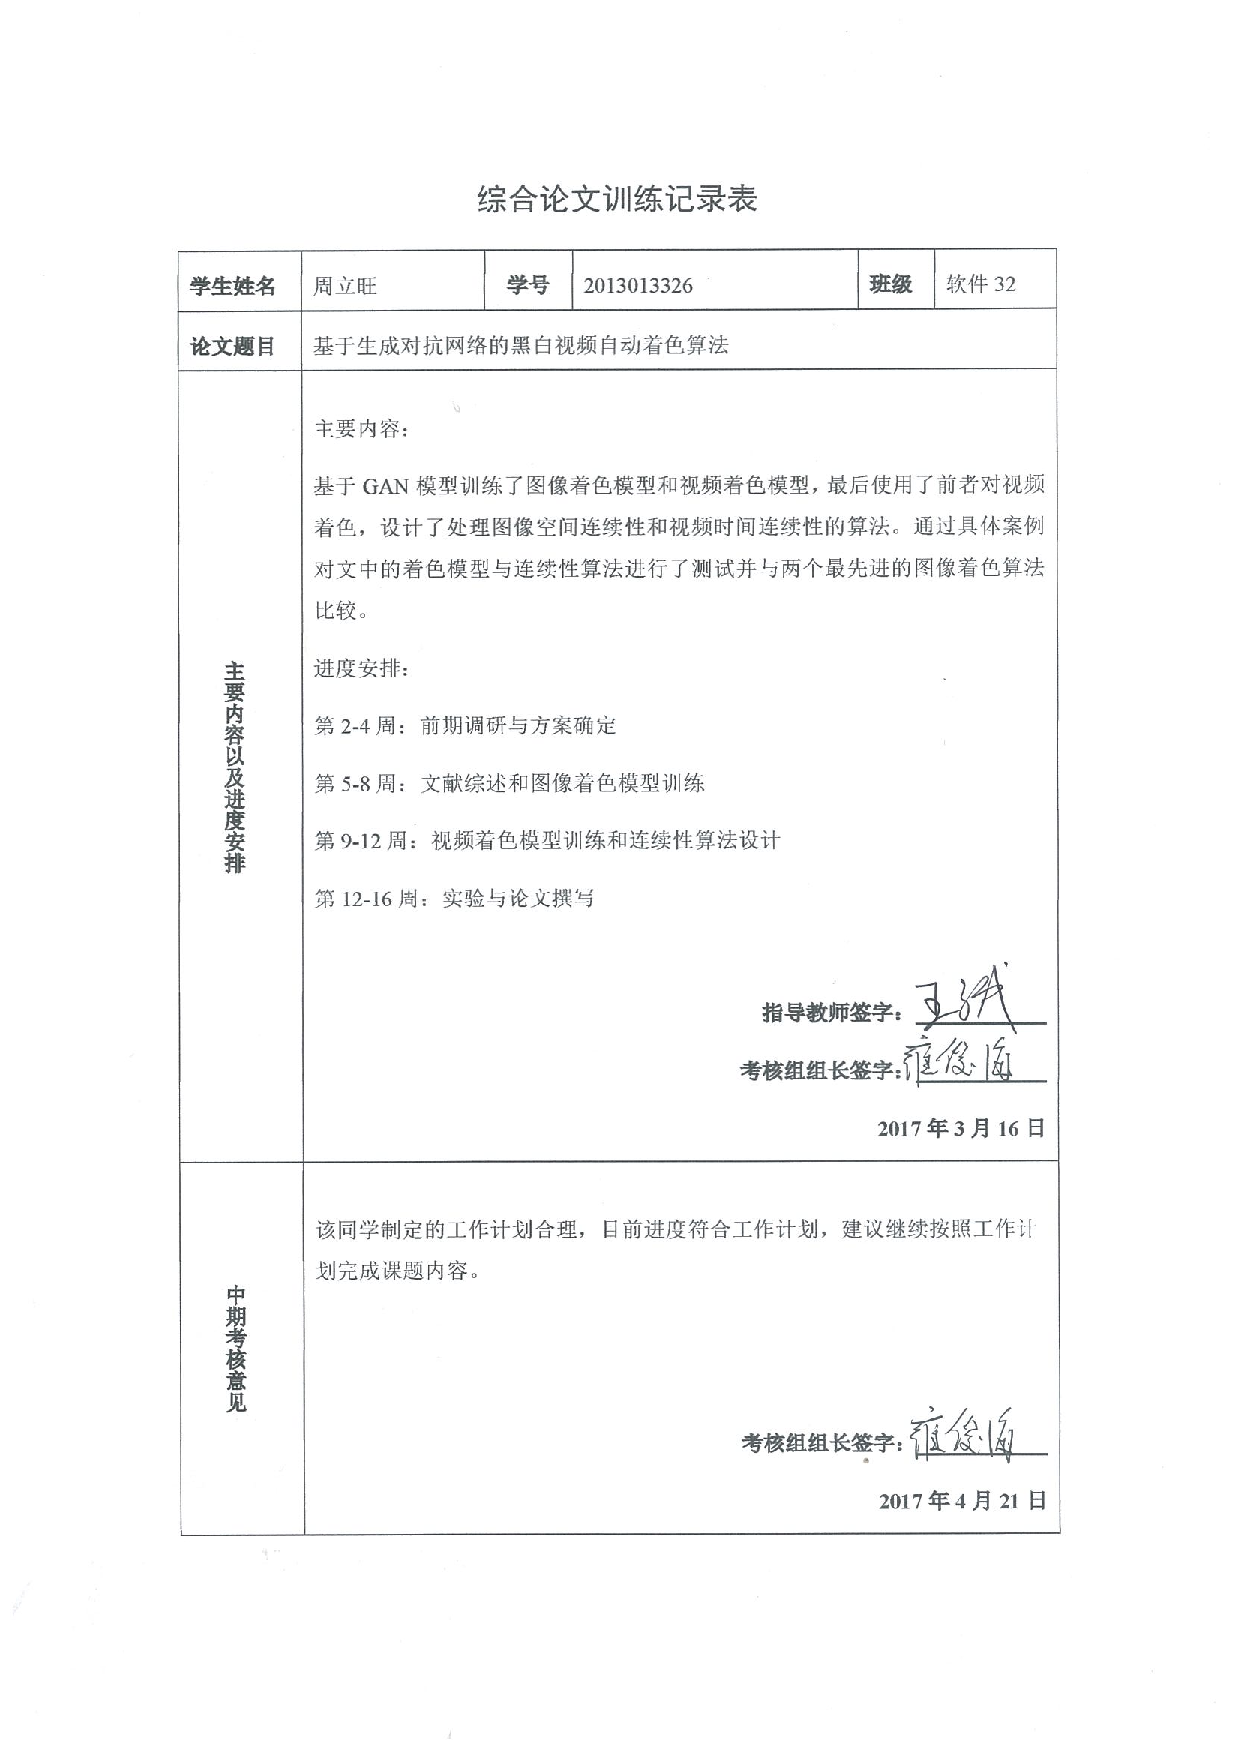
\includepdf[pages=-]{scan-record.pdf}
\end{document}
